% Build: latexmk -pdf -shell-escape report.tex   (minted, loaded by codespace.sty, needs -shell-escape)
\documentclass[twoside,final]{hcmut-report}
\usepackage{codespace}

\usepackage{gensymb,textcomp}
\usepackage{array,longtable,multicol,multirow,siunitx,tabularx}
\usepackage{enumitem}
\usepackage{caption,subcaption,float}
\usepackage[export]{adjustbox}
\usepackage{bm}
\usepackage[ruled,vlined,linesnumbered]{algorithm2e}
\usetikzlibrary{arrows.meta,positioning,shapes.geometric,fit,calc}
\usepackage[nameinlink]{cleveref}

\graphicspath{{../figures/}{graphics/}}

% Live numbers written by the notebook (section 8.1).
\newcommand{\NRaw}{32581}
\newcommand{\NClean}{32416}
\newcommand{\NDup}{165}
\newcommand{\NTrain}{25932}
\newcommand{\NTest}{6484}
\newcommand{\DefaultRate}{0.2187}
\newcommand{\BestModel}{Hist. Gradient Boosting}
\newcommand{\BestPrAuc}{0.9045}
\newcommand{\BestFTwo}{0.8132}
\newcommand{\BestRecall}{85.1\%}
\newcommand{\BestPrecision}{69.0\%}
\newcommand{\VeMs}{0.1}


\coursename{Machine Learning (CO3117)}
\reporttype{Assignment Report}
\title{Credit Risk Prediction with Traditional Machine Learning, Deep Learning and Bayesian Networks}
\advisor{& Dr. Le Thanh Sach &}
\stuname{%
  & Duong Nguyen Tan Dat & 2352222 \\
}

\AtBeginDocument{\counterwithin{lstlisting}{section}}
\AtBeginDocument{\counterwithin{algocf}{section}}

\newcommand{\code}[1]{\texttt{\detokenize{#1}}}
\newcommand{\Fbeta}{F_{\beta}}
\DeclareMathOperator*{\argmax}{arg\,max}
\DeclareMathOperator{\Pa}{Pa}
\newcommand{\pa}{\mathrm{pa}}

\begin{document}
\coverpage%

\section*{Member list \& workload}
\addcontentsline{toc}{section}{Member list \& workload}
\begin{center}
  \begin{tabular}{clcc}
    \toprule
    \textbf{No.} & \textbf{Full name} & \textbf{Student ID} & \textbf{Contribution} \\
    \midrule
    1 & Duong Nguyen Tan Dat & 2352222 & 100\% \\
    \bottomrule
  \end{tabular}
\end{center}

\noindent The group has a single member, who carried out every task listed below.

\begin{center}
  \small
  \begin{tabularx}{\linewidth}{lXc}
    \toprule
    \textbf{Work item} & \textbf{Description} & \textbf{Done} \\
    \midrule
    Dataset selection and EDA & Data quality audit, distributions, correlations, missing-value analysis & 100\% \\
    Traditional pipeline & Configurable preprocessing, six ablation suites, tuning of eight classifiers & 100\% \\
    Deep learning pipeline & Entity-embedding MLP (seven variants), TabNet, learned features & 100\% \\
    Bayesian network (extension) & From-scratch DAG, learning, exact and approximate inference & 100\% \\
    Engineering & Python package, unit tests, Colab notebook, GitHub repository & 100\% \\
    Report & This document & 100\% \\
    \bottomrule
  \end{tabularx}
\end{center}
\clearpage

\begin{abstract}
  This report predicts whether a borrower will default on a loan, using the public Credit Risk Dataset of \num{32581} loans.
Three approaches are built and compared under one evaluation protocol designed for an imbalanced problem in which a missed defaulter is costlier than a rejected applicant: models are ranked by PR-AUC and their decision thresholds are tuned for the F2 score.
First, a fully configurable traditional pipeline is evaluated through controlled ablations of imputation, outlier handling, encoding, scaling, dimensionality reduction and class-imbalance strategies, followed by the tuning of eight classifiers.
Second, a deep learning pipeline trains a multilayer perceptron with entity embeddings and TabNet.
Third, as the talented-engineering extension, a Bayesian network library is implemented from scratch, with Naive Bayes, TAN, BIC hill-climbing and expert structures, exact inference by variable elimination and approximate inference by rejection sampling, likelihood weighting and Gibbs sampling.
Histogram-based gradient boosting performs best, with a test PR-AUC of \BestPrAuc{}; at its F2-tuned threshold it detects \BestRecall{} of the defaulters with a precision of \BestPrecision{}, and neither a wider search nor stacking improves on it.
The entity-embedding network outperforms every linear model but not the tree ensembles.
The Bayesian networks are less accurate but fully interpretable: they answer diagnostic queries exactly, and comparing their answers with empirical frequencies reveals which independence assumptions the data contradict.
All experiments run end to end in a Google Colab notebook, and the code, features and report are available on GitHub.

\end{abstract}
\clearpage

\tableofcontents
\listoffigures
\listoftables
\listofalgorithms
\clearpage

\section{Introduction}
\label{sec:intro}

\subsection{Problem statement}
Before granting a loan, a lender must estimate how likely the applicant is to default, that is, to stop repaying.
Approving a future defaulter loses the principal, while rejecting a reliable applicant only loses the interest margin, so the two kinds of error have very different costs.
This report studies the problem as binary classification on the public Credit Risk Dataset \cite{kaggle_credit}.
Each of its \num{32581} records describes one applicant (age, income, employment length, home ownership, credit history) and one loan (purpose, grade, amount, interest rate, loan-to-income ratio).
The target \ident{loan_status} equals 1 when the loan defaulted.

The dataset meets the constraints of the assignment for tabular data.
It contains missing values (in \ident{person_emp_length} and \ident{loan_int_rate}), which calls for imputation.
It contains four categorical variables, which call for encoding.
It is large enough for reliable cross-validation and a held-out test set of \num{6484} loans.

\subsection{Objectives}
Following the assignment specification, the project pursues four objectives.
\begin{enumerate}
  \item \textbf{Traditional pipeline (mandatory).} Build a complete pipeline with exploratory data analysis, preprocessing, feature extraction and selection, model training and evaluation, where every step is configurable. Then measure the effect of each choice with controlled experiments.
  \item \textbf{Model comparison.} Tune and compare eight classical classifiers under one evaluation protocol designed for an imbalanced, cost-asymmetric problem.
  \item \textbf{Deep learning pipeline (bonus).} Train neural networks that learn their own representation of the tabular data (an entity-embedding MLP and TabNet), save the learned features, and compare them with the traditional pipeline.
  \item \textbf{Bayesian network (talented-engineering extension).} Implement a Bayesian network from scratch, with structure and parameter learning, exact inference (variable elimination) and approximate inference (rejection sampling, likelihood weighting, Gibbs sampling). Then apply it to the same prediction problem and to probabilistic reasoning about the causes of default.
\end{enumerate}

\subsection{Contributions}
\begin{itemize}
  \item A reusable Python package (\ident{modules/creditrisk}) that builds any pipeline variant from a declarative configuration. It is driven by a Google Colab notebook that runs end to end with \emph{Run all}.
  \item Six ablation studies on imputation, scaling, outliers and feature engineering, encoding, dimensionality reduction, and class imbalance, followed by grid-searched models with F2-tuned decision thresholds.
  \item A deep learning comparison with seven MLP variants and TabNet, and an analysis of the learned embeddings.
  \item A from-scratch Bayesian-network library, verified by unit tests against brute-force enumeration and scikit-learn's \ident{CategoricalNB}. It is used to compare four network structures and three sampling algorithms.
  \item Saved feature sets (\ident{.npy} and \ident{.h5}) for every pipeline, and a public GitHub repository.
\end{itemize}

\subsection{Deliverables and reproducibility}
The submission follows the required layout: \ident{notebooks/}, \ident{modules/}, \ident{reports/} and \ident{features/}.
\begin{itemize}[nosep]
  \item Source code: \url{https://github.com/datduongabc/credit-risk-classification}
  \item Colab notebook: \url{https://colab.research.google.com/github/datduongabc/credit-risk-classification/blob/main/notebooks/credit_risk_pipeline.ipynb}
\end{itemize}
The notebook clones the repository, installs the missing libraries and downloads the dataset from a public link, without mounting any personal storage.
Every number in this report is read from files that the notebook generates (\ident{reports/generated/}).
All randomness is seeded, so a re-run reproduces the tables; the deep models, whose results vary slightly across hardware and PyTorch builds, are reported as the mean and standard deviation over five seeds, so a run on another machine lands within the reported spread.

\subsection{Organization of the report}
\Cref{sec:eda} analyses the data and derives the preprocessing decisions.
\Cref{sec:method} presents the evaluation protocol and the three modelling approaches.
\Cref{sec:experiments} reports the experiments.
\Cref{sec:discussion} discusses strengths, limitations and threats to validity.
\Cref{sec:conclusion} concludes.
The appendix documents the code structure, the tests and the saved features.

\section{Dataset and exploratory data analysis}
\label{sec:eda}

\subsection{The Credit Risk Dataset}
The dataset \cite{kaggle_credit} has \num{32581} rows and 12 columns: seven numeric features, four categorical features and the binary target (\cref{tab:overview}).
The dataset is released under CC0 (public domain).
The notebook downloads it from a public mirror in the project's GitHub releases, falls back to Kaggle, and verifies its SHA-256 checksum, so every run uses exactly the same file.

\begin{table}[H]
  \centering
  \small
  \begin{tabularx}{\linewidth}{lX}
    \toprule
    \textbf{Column} & \textbf{Meaning} \\
    \midrule
    \ident{person_age} & Age of the applicant (years) \\
    \ident{person_income} & Annual income (USD) \\
    \ident{person_home_ownership} & RENT, MORTGAGE, OWN or OTHER \\
    \ident{person_emp_length} & Employment length (years) \\
    \ident{loan_intent} & Purpose: EDUCATION, MEDICAL, VENTURE, PERSONAL, DEBTCONSOLIDATION, HOMEIMPROVEMENT \\
    \ident{loan_grade} & Lender's risk grade from A (best) to G (worst) \\
    \ident{loan_amnt} & Requested amount (USD) \\
    \ident{loan_int_rate} & Interest rate (\%) \\
    \ident{loan_percent_income} & Loan amount divided by annual income \\
    \ident{cb_person_default_on_file} & Whether the credit bureau records a past default (Y/N) \\
    \ident{cb_person_cred_hist_length} & Length of the credit history (years) \\
    \ident{loan_status} & \textbf{Target}: 1 = default, 0 = non-default \\
    \bottomrule
  \end{tabularx}
  \caption{Columns of the Credit Risk Dataset.}
  \label{tab:columns}
\end{table}

\begin{table}[H]
\centering
\small
\begin{adjustbox}{max width=\linewidth}
\begin{tabular}{llrrr}
\toprule
column & type & missing & missing (\%) & unique \\
\midrule
person\_age & numeric & 0 & 0.00 & 58 \\
person\_income & numeric & 0 & 0.00 & 4295 \\
person\_home\_ownership & categorical & 0 & 0.00 & 4 \\
person\_emp\_length & numeric & 895 & 2.75 & 36 \\
loan\_intent & categorical & 0 & 0.00 & 6 \\
loan\_grade & categorical & 0 & 0.00 & 7 \\
loan\_amnt & numeric & 0 & 0.00 & 753 \\
loan\_int\_rate & numeric & 3116 & 9.56 & 348 \\
loan\_status & categorical & 0 & 0.00 & 2 \\
loan\_percent\_income & numeric & 0 & 0.00 & 77 \\
cb\_person\_default\_on\_file & categorical & 0 & 0.00 & 2 \\
cb\_person\_cred\_hist\_length & numeric & 0 & 0.00 & 29 \\
\bottomrule
\end{tabular}
\end{adjustbox}
\caption{Columns of the raw dataset.}
\label{tab:overview}
\end{table}


\subsection{Data quality}
\label{subsec:quality}

\paragraph{Duplicates.}
\num{165} rows are exact duplicates of other rows.
They are removed, because duplicates inflate the apparent sample size and can land on both sides of the train/test split.

\paragraph{Impossible values.}
Five applicants are older than 100 (two of them are 144), and two report 123 years of employment while being 21 and 22 years old (\cref{fig:boxplots}).
These are data-entry errors, not genuine extremes.
We turn them into missing values, using the rules age $> 100$ and employment length $>$ age $-$ 14, and let the imputer fill them.
The rules are deterministic and row-local, so applying them before the split cannot leak information.

\begin{figure}[H]
  \centering
  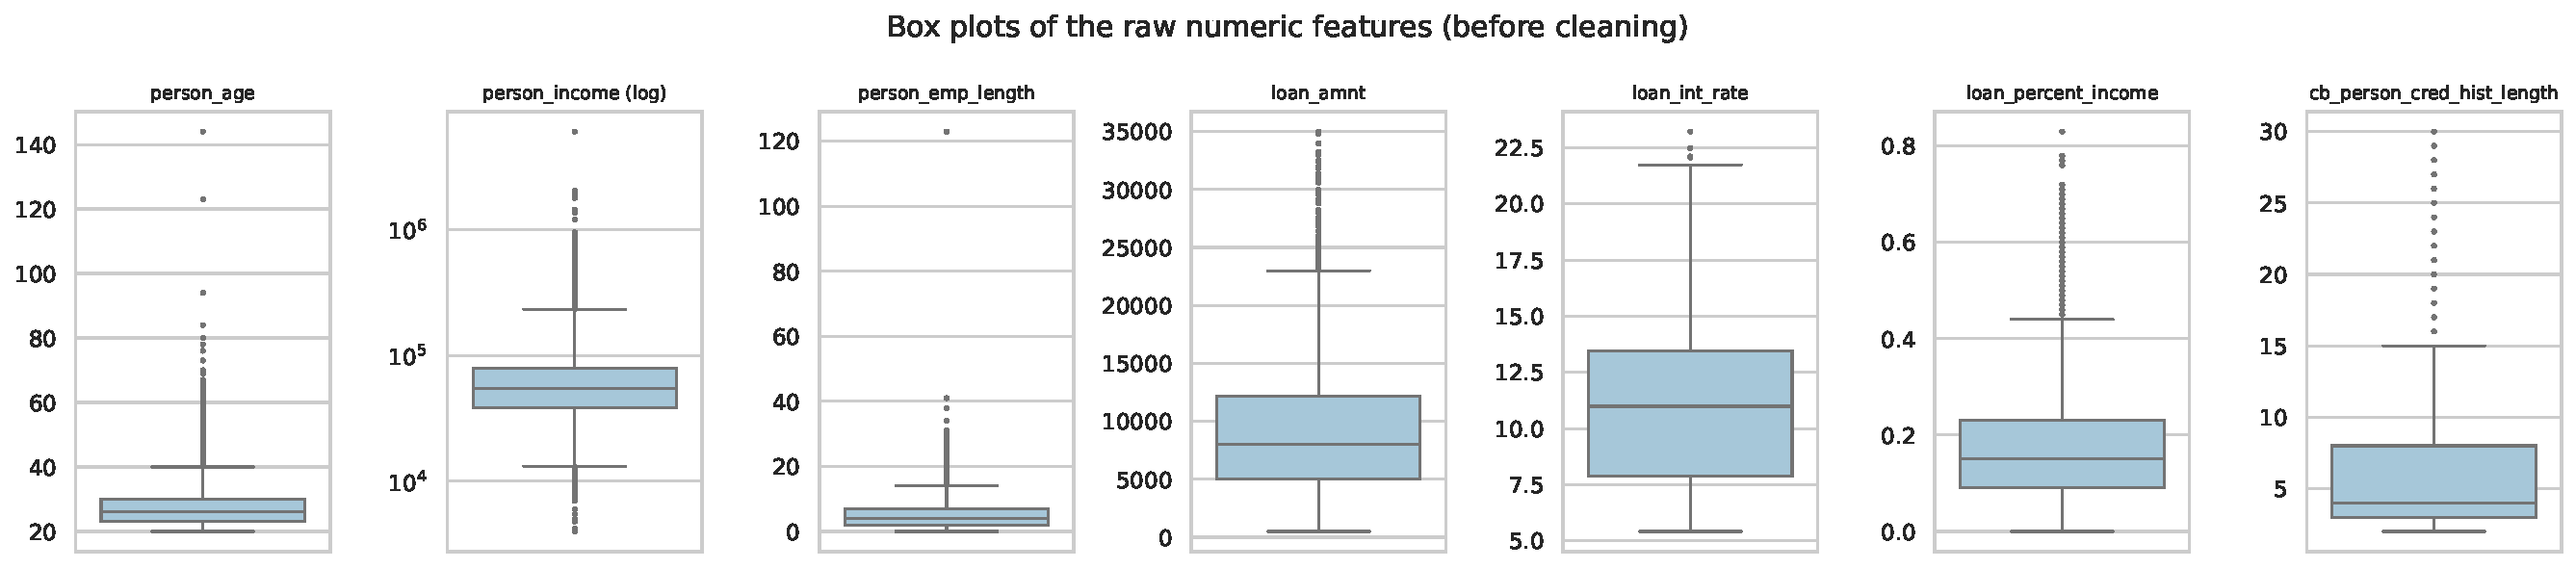
\includegraphics[width=\linewidth]{eda_boxplots.pdf}
  \caption{Box plots of the raw numeric features. Note the impossible ages and employment lengths, and the heavy right tails of income and amounts.}
  \label{fig:boxplots}
\end{figure}

\paragraph{Skewness and genuine outliers.}
Income is extremely right-skewed (skewness 32.9, median \$55{,}000, maximum \$6{,}000{,}000).
The loan amount, loan-to-income ratio and credit-history length also have long right tails.
Unlike the impossible values, these are plausible and are kept.
Whether to winsorize them or log-transform them is treated as a pipeline option and decided experimentally (\cref{tab:suite_outlier_fe}).

\begin{table}[H]
\centering
\scriptsize
\begin{adjustbox}{max width=\linewidth}
\begin{tabular}{lrrrrrrrr}
\toprule
feature & mean & std & min & 1\% & 50\% & 99\% & max & skew \\
\midrule
person\_age & 27.73 & 6.35 & 20.00 & 21.00 & 26.00 & 50.00 & 144.00 & 2.58 \\
person\_income & 66074.85 & 61983.12 & 4000.00 & 14400.00 & 55000.00 & 225200.00 & 6000000.00 & 32.87 \\
person\_emp\_length & 4.79 & 4.14 & 0.00 & 0.00 & 4.00 & 18.00 & 123.00 & 2.61 \\
loan\_amnt & 9589.37 & 6322.09 & 500.00 & 1000.00 & 8000.00 & 29800.00 & 35000.00 & 1.19 \\
loan\_int\_rate & 11.01 & 3.24 & 5.42 & 5.42 & 10.99 & 18.62 & 23.22 & 0.21 \\
loan\_percent\_income & 0.17 & 0.11 & 0.00 & 0.02 & 0.15 & 0.50 & 0.83 & 1.06 \\
cb\_person\_cred\_hist\_length & 5.80 & 4.06 & 2.00 & 2.00 & 4.00 & 17.00 & 30.00 & 1.66 \\
\bottomrule
\end{tabular}
\end{adjustbox}
\caption{Descriptive statistics of the numeric features (raw data).}
\label{tab:numeric}
\end{table}


\subsection{Target distribution}
Only 21.8\% of the loans defaulted (\cref{fig:target}).
This moderate imbalance drives three design decisions:
\begin{itemize}[nosep]
  \item the split and every cross-validation fold are stratified;
  \item accuracy is not used for model selection, PR-AUC and F2 are used instead (\cref{subsec:protocol});
  \item class weights, SMOTE and under-sampling are compared as remedies.
\end{itemize}

\begin{figure}[H]
  \centering
  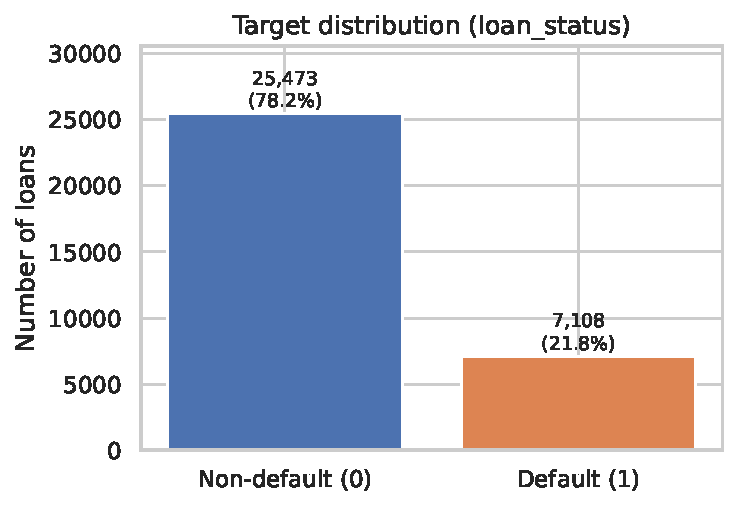
\includegraphics[width=0.5\linewidth]{eda_target.pdf}
  \caption{Distribution of the target \ident{loan_status}.}
  \label{fig:target}
\end{figure}

\subsection{Numeric features}
\Cref{fig:numeric} compares the class-conditional distributions after cleaning.
Three features separate the classes clearly.
\begin{itemize}[nosep]
  \item \ident{loan_percent_income}: defaulters typically borrow more than 30\% of their income, while most non-defaulters stay below 20\%.
  \item \ident{loan_int_rate}: defaulters concentrate at rates above 14\%.
  \item \ident{person_income}: defaulters have lower incomes (on the log scale).
\end{itemize}
Age, employment length and credit-history length have nearly identical distributions in both classes.
Most applicants are young (median age 26; 76\% are 30 or younger).

\begin{figure}[H]
  \centering
  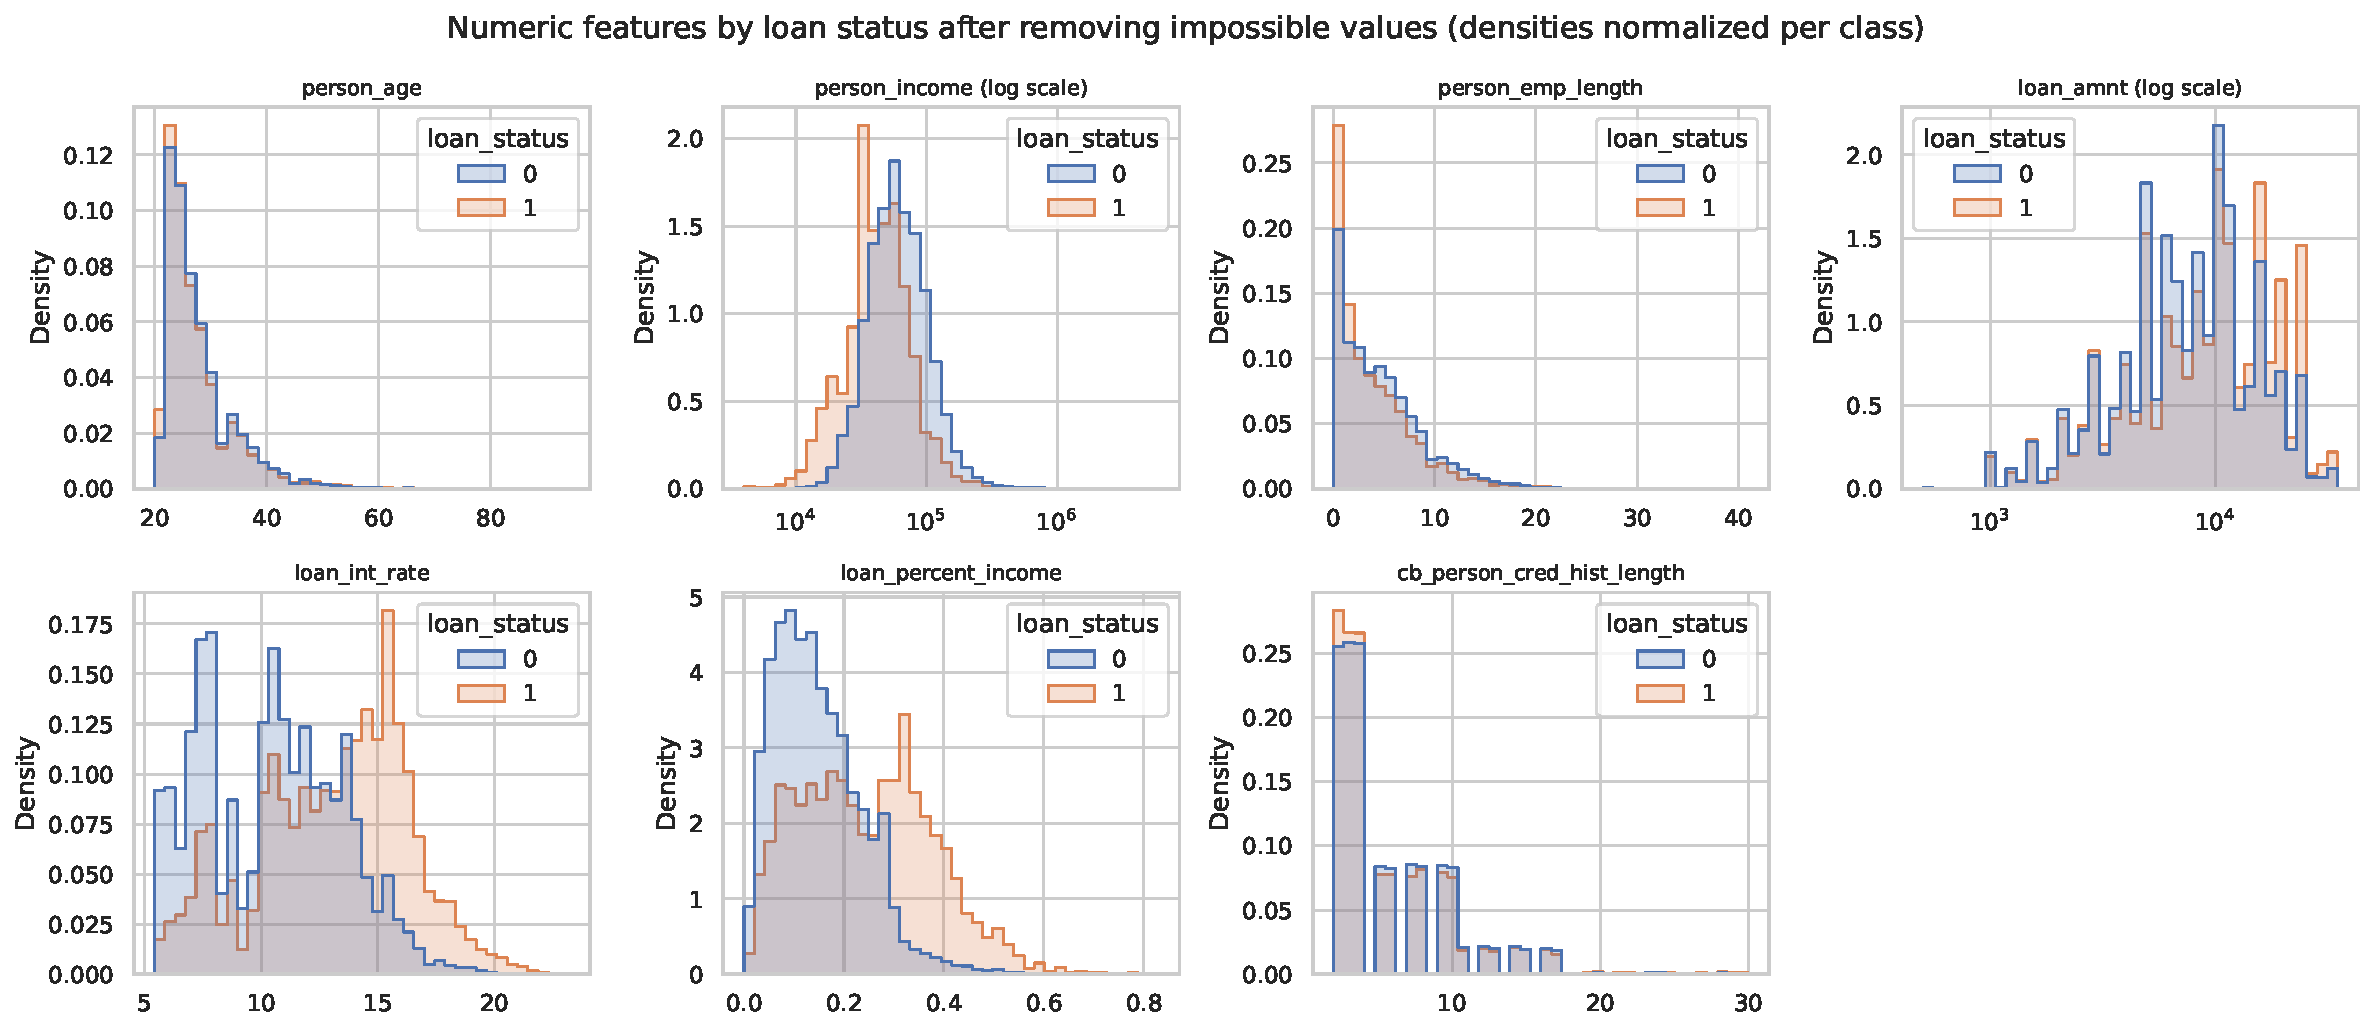
\includegraphics[width=\linewidth]{eda_numeric.pdf}
  \caption{Class-conditional distributions of the numeric features (after removing impossible values; densities normalized per class).}
  \label{fig:numeric}
\end{figure}

\subsection{Categorical features}
\Cref{fig:categorical} shows the frequency of each category and its default rate.
\begin{itemize}[nosep]
  \item \textbf{Loan grade} is the strongest categorical signal. The default rate rises monotonically from 10.0\% (A) and 16.3\% (B) to 59.0\% (D) and 98.4\% (G). The jump between C and D is the largest. The order supports an ordinal encoding.
  \item \textbf{Home ownership}: renters default four times as often as owners (31.6\% versus 7.5\%). Mortgage holders sit in between (12.6\%). The OTHER category is rare (107 rows).
  \item \textbf{Past default on file}: 37.8\% of applicants with a recorded past default default again, against 18.4\% of the others.
  \item \textbf{Loan intent} has a weaker effect, from 14.8\% (VENTURE) to 28.6\% (DEBTCONSOLIDATION).
\end{itemize}

\begin{figure}[H]
  \centering
  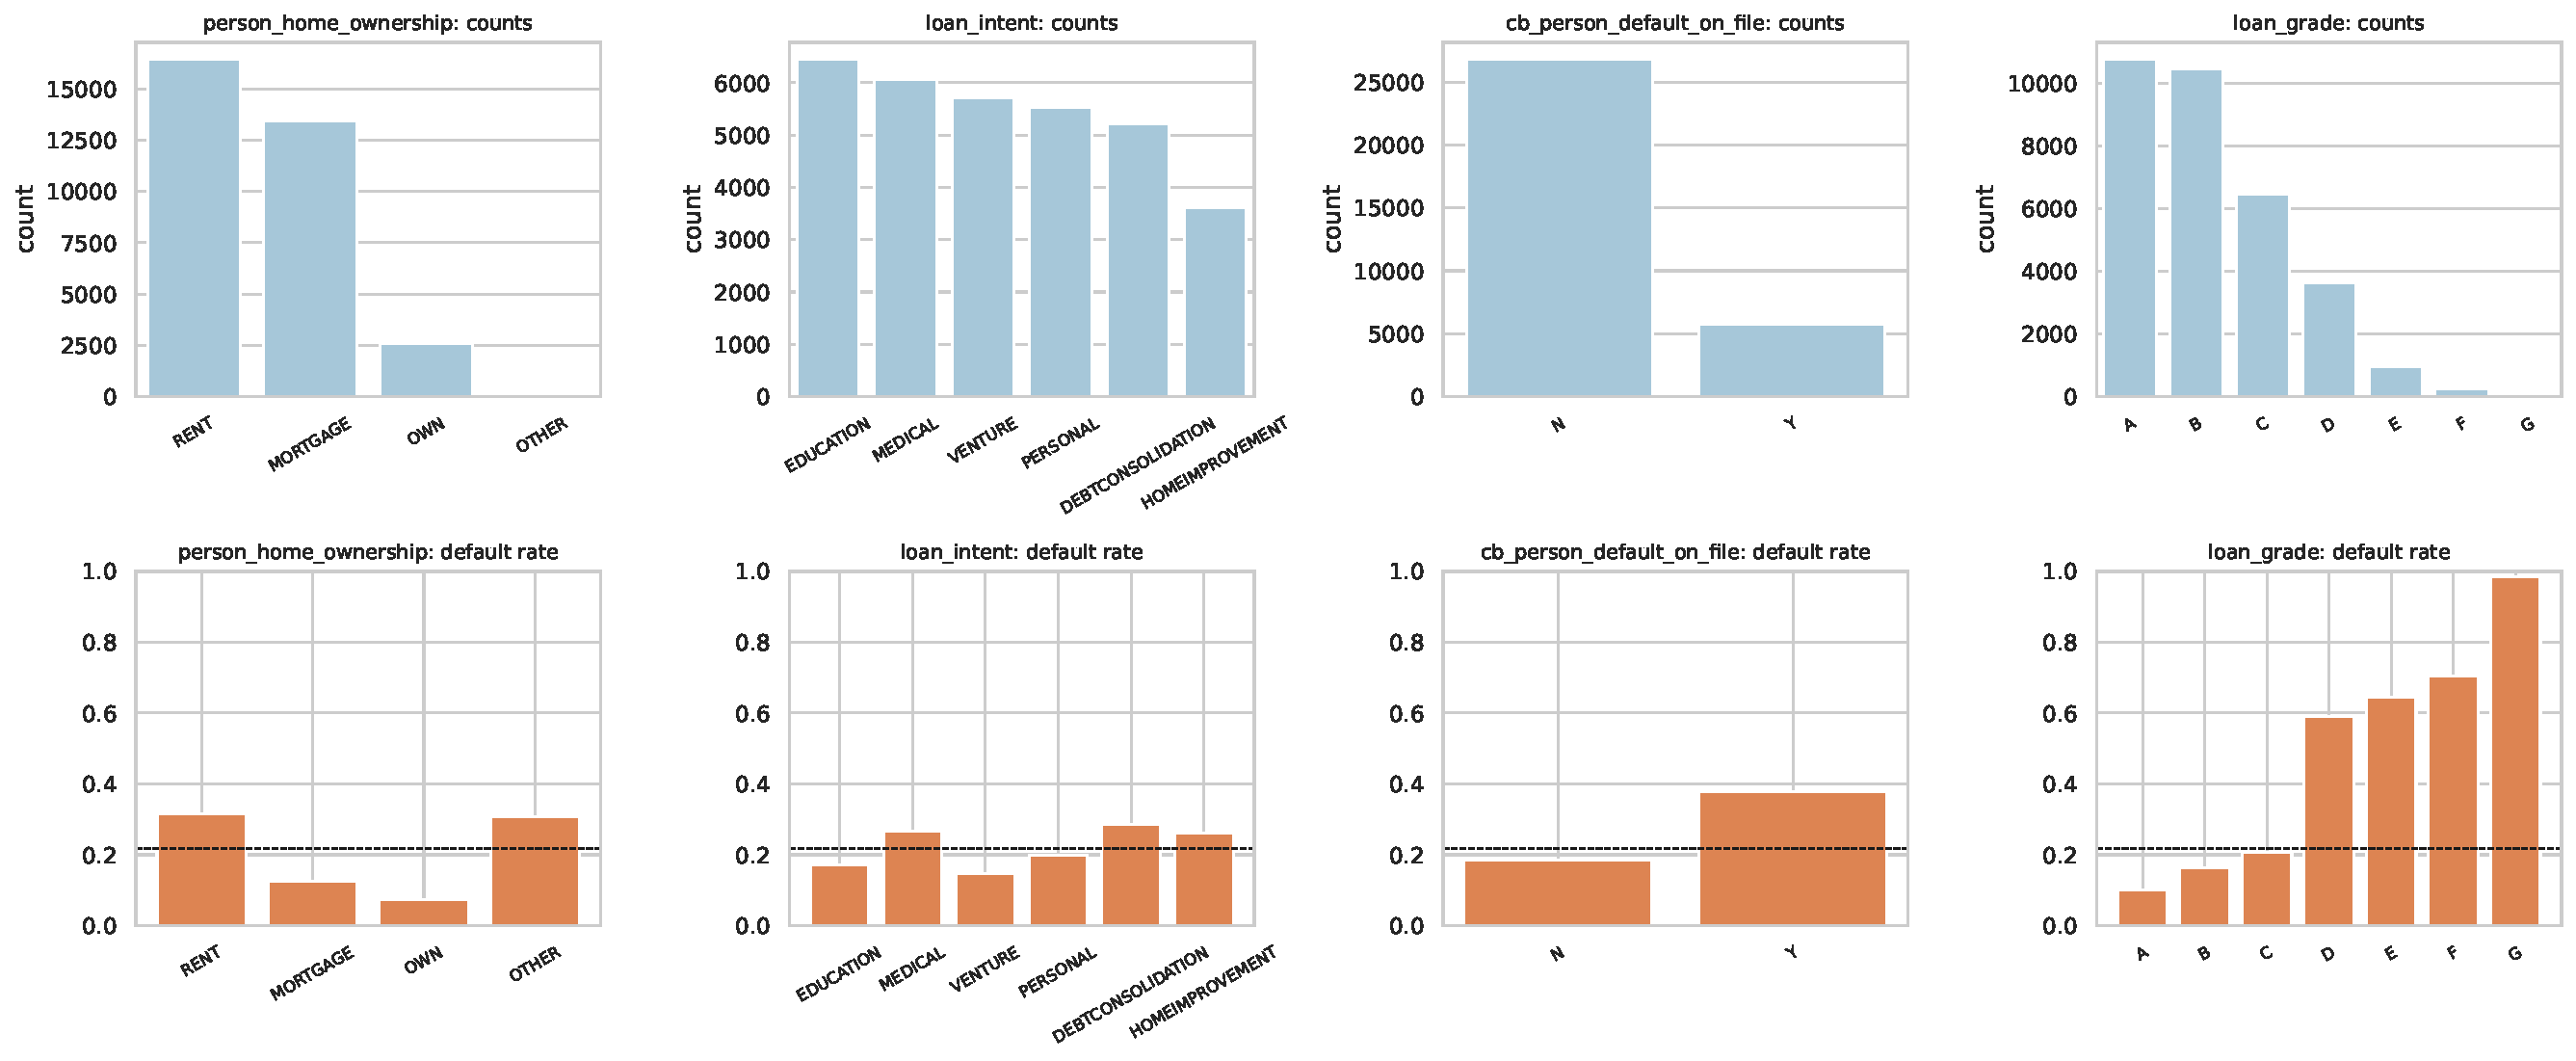
\includegraphics[width=\linewidth]{eda_categorical.pdf}
  \caption{Categorical features: counts (top) and default rate per category (bottom; the dashed line is the overall rate).}
  \label{fig:categorical}
\end{figure}

\subsection{Correlations and feature relevance}
The Spearman correlation matrix (\cref{fig:correlation}) reveals three strongly related pairs:
\begin{itemize}[nosep]
  \item the interest rate and the grade ($\rho = 0.95$): the lender prices loans by grade;
  \item age and credit-history length ($\rho = 0.81$);
  \item the loan amount and the loan-to-income ratio ($\rho = 0.65$).
\end{itemize}
These redundancies matter for linear models (collinearity), and they explain why a single grade-related feature carries most of the signal.
The features most correlated with the target are the grade (0.33), the interest rate (0.32), the loan-to-income ratio (0.32) and the income ($-0.27$).

Mutual information (\cref{fig:mi}) also captures non-monotone dependence.
It ranks income first, followed by the loan-to-income ratio, the grade and the interest rate.
Age and credit-history length carry almost no information on their own.
The scatter plot in \cref{fig:burden} shows that the classes overlap strongly in any single feature, but that defaults concentrate where low income meets a high loan-to-income ratio.
This is an interaction that tree ensembles can capture directly.

\begin{figure}[H]
  \centering
  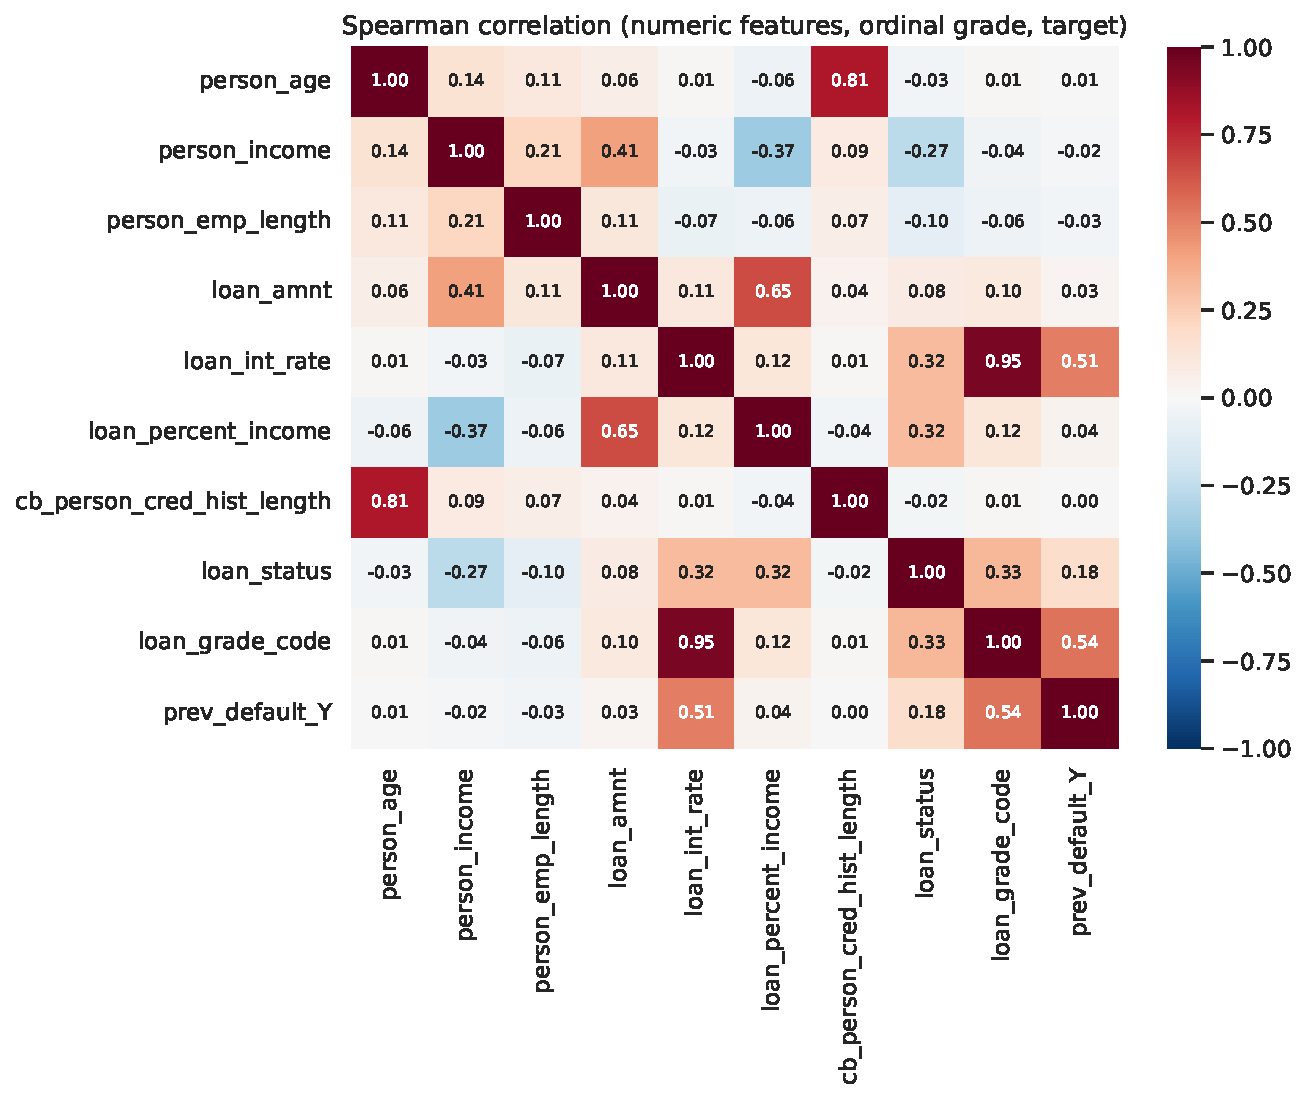
\includegraphics[width=0.75\linewidth]{eda_correlation.pdf}
  \caption{Spearman correlations between numeric features, the ordinal grade, the past-default flag and the target.}
  \label{fig:correlation}
\end{figure}

\begin{figure}[H]
  \centering
  \begin{subfigure}{0.49\linewidth}
    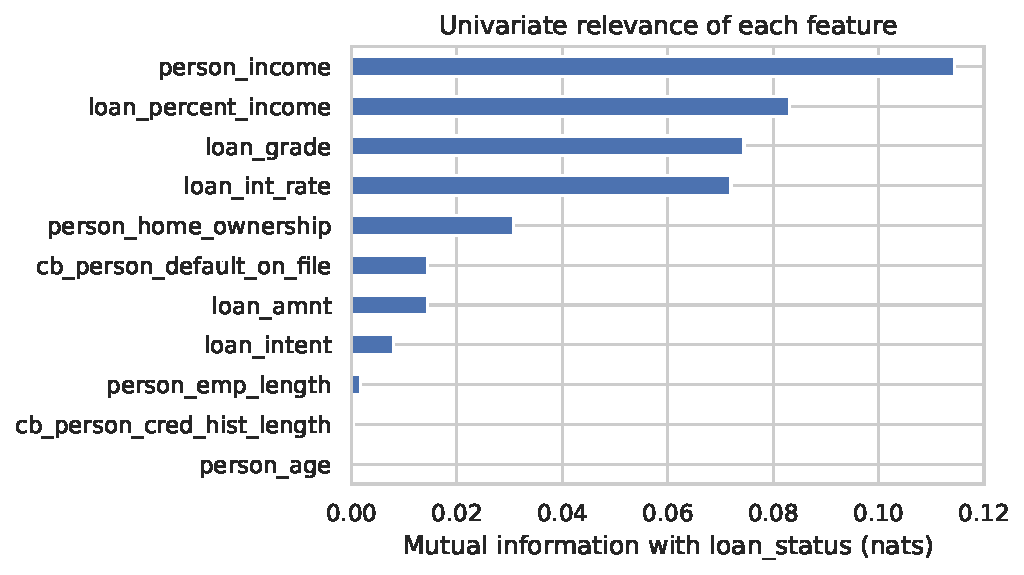
\includegraphics[width=\linewidth]{eda_mutual_info.pdf}
    \caption{Mutual information with the target.}
    \label{fig:mi}
  \end{subfigure}
  \hfill
  \begin{subfigure}{0.49\linewidth}
    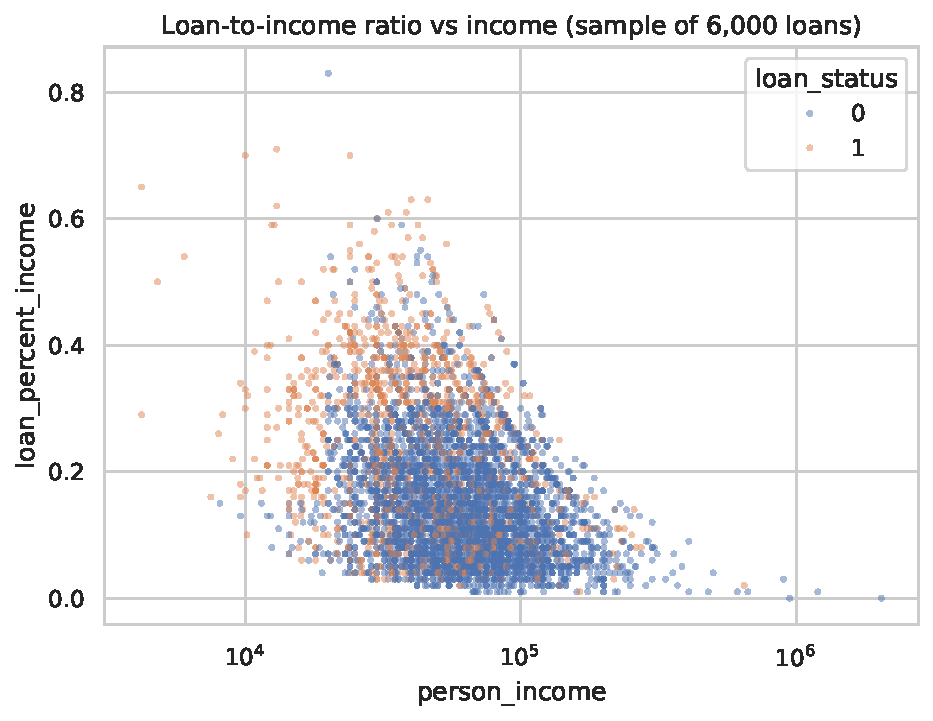
\includegraphics[width=\linewidth]{eda_burden.pdf}
    \caption{Loan-to-income ratio versus income.}
    \label{fig:burden}
  \end{subfigure}
  \caption{Relevance of individual features and an example interaction.}
\end{figure}

\subsection{Missing values}
\label{subsec:missing}
Two columns have missing values: \ident{person_emp_length} (895 rows, 2.75\%) and \ident{loan_int_rate} (\num{3116} rows, 9.56\%).
They are missing together in only 68 rows.
\Cref{fig:missing} shows that the two columns behave differently.
\begin{itemize}
  \item A missing \textbf{interest rate} is uninformative. Loans with a missing rate default at 20.7\%, against 21.9\% for loans with an observed rate, and the share of missing rates is flat across grades. This is consistent with \emph{missing completely at random}. Because the rate is almost determined by the grade (\cref{fig:rate_grade}), the grade-wise median is a natural imputation.
  \item A missing \textbf{employment length} is informative. These applicants default at 31.5\%, against 21.5\% otherwise. The missingness itself carries signal, which motivates the optional missing-value indicators.
\end{itemize}

\begin{figure}[H]
  \centering
  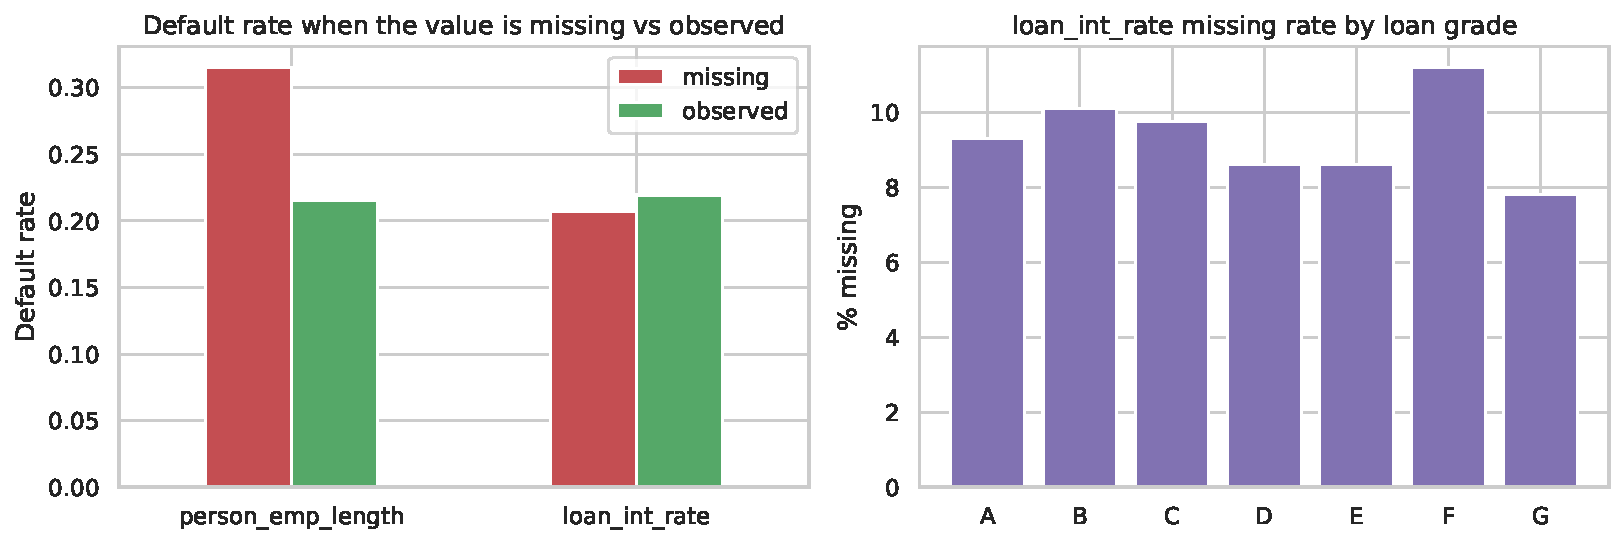
\includegraphics[width=\linewidth]{eda_missing.pdf}
  \caption{Left: default rate when a value is missing or observed. Right: missing share of \ident{loan_int_rate} per grade.}
  \label{fig:missing}
\end{figure}

\begin{figure}[H]
  \centering
  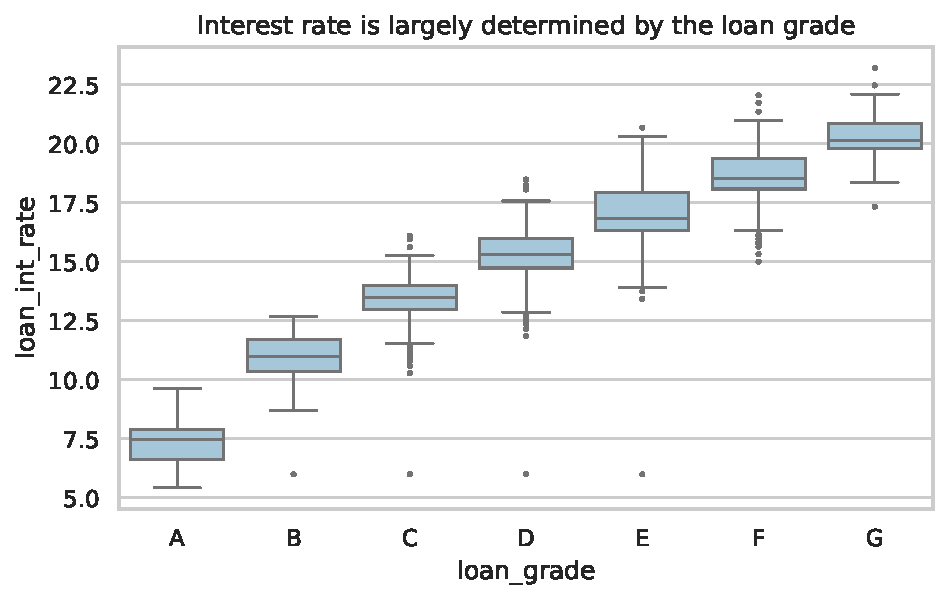
\includegraphics[width=0.6\linewidth]{eda_rate_grade.pdf}
  \caption{Interest rate by loan grade: the grade almost determines the rate.}
  \label{fig:rate_grade}
\end{figure}

\subsection{Implications for the pipeline}
\Cref{tab:eda_decisions} summarizes how the findings shape the pipeline.

\begin{table}[H]
  \centering
  \small
  \begin{tabularx}{\linewidth}{XX}
    \toprule
    \textbf{Finding} & \textbf{Pipeline decision} \\
    \midrule
    165 duplicates, 7 impossible values & Rule-based cleaning before the split; impossible values become missing \\
    21.8\% defaults, asymmetric error costs & Stratification; PR-AUC for selection and an F2-tuned threshold; class-imbalance remedies compared \\
    Interest rate determined by grade & Grade-wise median imputation as an option \\
    Informative missing employment length & Optional missing-value indicators \\
    Heavy right tails (income, amounts) & IQR winsorizing or log transform as options; log features in feature engineering \\
    Monotone default rate across grades & Ordinal versus one-hot grade encoding compared \\
    Very different scales (income vs ratios) & Scaler choice compared, essential for k-NN and SVM \\
    Correlated features, only 11 inputs & PCA and feature selection tested, with little redundancy expected \\
    Interactions (income $\times$ burden, grade $\times$ housing) & Tree ensembles and neural networks expected to do well \\
    \bottomrule
  \end{tabularx}
  \caption{From EDA findings to pipeline options.}
  \label{tab:eda_decisions}
\end{table}

\section{Methodology}
\label{sec:method}

This section describes the evaluation protocol shared by all experiments and then the three modelling approaches.
\Cref{fig:architecture} gives an overview of how the data flows through the project.

\begin{figure}[H]
  \centering
  \begin{tikzpicture}[
      font=\footnotesize,
      box/.style={draw, rounded corners, align=center, minimum height=1.1cm, fill=#1},
      box/.default=gray!12,
      arr/.style={-{Stealth[length=2mm]}, thick}
    ]
    % Row 1: shared data preparation
    \node[box, text width=3.4cm] (raw) at (-5, 0) {Raw CSV\\Kaggle, 32{,}581 loans};
    \node[box, text width=3.4cm] (clean) at (0, 0) {Rule-based cleaning\\duplicates, impossible values};
    \node[box, text width=3.4cm] (split) at (5, 0) {Stratified split\\80\% train / 20\% test};
    \draw[arr] (raw) -- (clean);
    \draw[arr] (clean) -- (split);
    % Row 2: the three model families
    \node[box=blue!8, text width=4.3cm, minimum height=2.2cm] (trad) at (-5, -3)
      {\textbf{Traditional pipeline}\\impute, engineer, clip, encode, scale, select / PCA, resample, classifier (8 models)};
    \node[box=orange!12, text width=4.3cm, minimum height=2.2cm] (dl) at (0, -3)
      {\textbf{Deep learning pipeline}\\impute and scale numerics, integer codes, entity embeddings, MLP / TabNet};
    \node[box=green!10, text width=4.3cm, minimum height=2.2cm] (bn) at (5, -3)
      {\textbf{Bayesian network}\\quantile bins, structure learning, CPTs, exact and approximate inference};
    \coordinate (bus) at (0, -1.25);
    \draw[thick] (split.south) |- (bus -| trad.north);
    \draw[thick] (bus -| split.south) -- (bus -| trad.north);
    \draw[arr] (bus -| trad.north) -- (trad.north);
    \draw[arr] (bus -| dl.north) -- (dl.north);
    \draw[arr] (bus -| bn.north) -- (bn.north);
    % Row 3: shared evaluation and outputs
    \node[box, minimum width=14.2cm] (eval) at (0, -6.2)
      {\textbf{Common evaluation}: 5-fold stratified CV on the training set, decision threshold tuned for F2,\\
       one final test-set evaluation (PR-AUC, ROC-AUC, F2, recall, precision); features saved as \texttt{.npy} / \texttt{.h5}};
    \draw[arr] (trad.south) -- (trad.south |- eval.north);
    \draw[arr] (dl.south) -- (dl.south |- eval.north);
    \draw[arr] (bn.south) -- (bn.south |- eval.north);
  \end{tikzpicture}
  \caption{Overview of the project: one cleaned and split dataset feeds three model families that share the same evaluation protocol.}
  \label{fig:architecture}
\end{figure}

\subsection{Evaluation protocol}
\label{subsec:protocol}

\paragraph{Data split.}
After rule-based cleaning (\Cref{subsec:quality}), the data are split once into a stratified training set (80\%) and test set (20\%) with a fixed seed.
Every learned step (imputation statistics, scaling parameters, PCA axes, discretization bins, network weights, CPTs, decision thresholds) is estimated on training data only.
The test set is used once per final model.

\paragraph{Cross-validation.}
Model selection uses 5-fold stratified cross-validation on the training set.
Because every preprocessing step lives inside one pipeline object, it is refitted on each training fold, so the validation fold never leaks into the preprocessing statistics.

\paragraph{Metrics.}
Let $TP, FP, FN, TN$ count the outcomes for the positive class (default).
We report
\begin{align}
  \text{precision} &= \frac{TP}{TP + FP}, &
  \text{recall} &= \frac{TP}{TP + FN}, &
  \Fbeta &= \frac{(1 + \beta^2)\,\text{precision}\cdot\text{recall}}{\beta^2\,\text{precision} + \text{recall}},
  \label{eq:fbeta}
\end{align}
together with accuracy, the area under the ROC curve (ROC-AUC) and the area under the precision-recall curve (PR-AUC, computed as average precision).

\paragraph{Why PR-AUC and F2 instead of accuracy or recall alone.}
Defaults make up only 21.8\% of the loans, so the trivial ``never default'' rule already reaches 78\% accuracy.
For a lender, a missed defaulter (false negative) loses the principal, whereas a rejected good applicant (false positive) loses only the interest margin.
Recall on the default class is therefore the quantity of interest, but recall alone is degenerate: flagging every applicant gives recall 1.
We consequently
\begin{enumerate}[nosep]
  \item rank models and select hyper-parameters by \textbf{PR-AUC}, a threshold-free measure that, unlike ROC-AUC, is sensitive to performance on the minority class \cite{saito2015}; and
  \item choose each model's operating threshold to maximize \textbf{F2} ($\beta = 2$ in \cref{eq:fbeta}), which weights recall twice as much as precision \cite{rijsbergen1979}.
\end{enumerate}
The threshold is tuned by internal cross-validation on the training set (\ident{TunedThresholdClassifierCV}) for the traditional models, and on a held-out 15\% validation split of the training set for the neural networks and Bayesian networks.

\subsection{Traditional machine learning pipeline}
\label{subsec:trad}

The pipeline is assembled by a single function from a declarative \ident{PipelineConfig}, shown in \cref{lst:config}.
All components are standard scikit-learn \cite{sklearn} or imbalanced-learn \cite{imblearn} classes, except two small transformers that have no library equivalent: grade-wise median imputation and IQR clipping.

\begin{listing}[H]
  \begin{minted}[fontsize=\footnotesize, frame=lines, bgcolor=gray!5]{python}
@dataclass(frozen=True)
class PipelineConfig:
    imputer: str = "median"          # mean | median | group_median | knn | iterative
    add_indicator: bool = False      # append missing-value indicator columns
    feature_engineering: bool = False
    outlier: str = "none"            # none | clip_iqr | log
    grade_encoding: str = "ordinal"  # ordinal | onehot
    scaler: str = "standard"         # none | standard | minmax | robust
    feature_range: tuple = (0.0, 1.0)  # used by MinMaxScaler
    select_k: int | None = None      # SelectKBest(mutual information)
    pca_variance: float | None = None  # e.g. 0.90, 0.95
    resampler: str = "none"          # none | smote | undersample
    class_weight: str | None = None  # None | "balanced"
    model: str = "logreg"            # one of the 8 classifiers below
    model_params: dict = field(default_factory=dict)

pipe = build_pipeline(PipelineConfig(imputer="group_median", scaler="minmax",
                                     feature_range=(-1, 1), pca_variance=0.95, model="svm"))
  \end{minted}
  \caption{Every pipeline step is selected through one configuration object.}
  \label{lst:config}
\end{listing}

\subsubsection{Missing-value imputation}
Five strategies are available.
\emph{Mean} and \emph{median} imputation replace a missing value by a training statistic of its column.
\emph{Grade-wise median} imputation fills \ident{loan_int_rate} with the median rate of the applicant's loan grade, which the EDA shows to be the main driver of the rate (\cref{fig:rate_grade}).
\emph{KNN} imputation \cite{troyanskaya2001} averages the five nearest neighbours in standardized feature space.
\emph{Iterative} imputation (MICE) \cite{mice} regresses each incomplete column on the others in round-robin fashion.
Optionally, binary missing-value indicators are appended so that the model can exploit informative missingness \cite{rubin1987}.

\subsubsection{Feature engineering and outliers}
Four domain features can be added: $\log(1+\text{income})$, $\log(1+\text{amount})$, income per year of credit history, and the product of the interest rate and the loan-to-income ratio, which approximates the repayment burden.
Outliers are handled by IQR winsorizing, which clips every value $x$ of a column to $[Q_1 - 1.5\,\mathrm{IQR},\; Q_3 + 1.5\,\mathrm{IQR}]$ with quartiles learned on the training fold, or by a $\log(1+x)$ transform of all numeric columns.

\subsubsection{Encoding and scaling}
Nominal variables (\ident{person_home_ownership}, \ident{loan_intent}, \ident{cb_person_default_on_file}) are one-hot encoded.
The loan grade has a natural order A~$<$~B~$<\dots<$~G, so it can be encoded either ordinally (0--6) or one-hot.
Numeric features can be standardized ($z = (x - \mu)/\sigma$), min-max scaled to a configurable range $[a, b]$ via $x' = a + (b - a)(x - x_{\min})/(x_{\max} - x_{\min})$, or robust-scaled with the median and IQR.

\subsubsection{Feature selection and dimensionality reduction}
\ident{SelectKBest} keeps the $k$ encoded features with the highest mutual information with the target.
PCA \cite{jolliffe2016} projects the scaled features onto the leading principal components that together retain a chosen fraction of the variance (80\%, 90\%, 95\% or 99\%).

\subsubsection{Class imbalance}
Three remedies are compared: class weights inversely proportional to class frequency ($w_c = n / (2 n_c)$), SMOTE \cite{smote}, which synthesizes minority samples by interpolating between minority neighbours, and random under-sampling of the majority class.
Resampling is applied only to the training folds (it is a pipeline step that is skipped at prediction time).

\subsubsection{Classifiers}
\Cref{tab:classifiers} lists the eight classifiers.
Six of them are suggested by the assignment; Gaussian Naive Bayes and histogram-based gradient boosting are added as a probabilistic baseline and as a strong modern tree ensemble.

\begin{table}[H]
  \centering
  \small
  \begin{tabularx}{\linewidth}{lX}
    \toprule
    \textbf{Classifier} & \textbf{Decision function / idea} \\
    \midrule
    Logistic Regression & $P(y=1 \mid \bm{x}) = \sigma(\bm{w}^\top \bm{x} + b)$, $L_2$-regularized log-loss with strength $1/C$ \\
    Linear SVM & Hinge loss with a linear decision boundary \\
    SVM (RBF) & Maximum-margin classifier with kernel $k(\bm{x}, \bm{x}') = \exp(-\gamma \lVert \bm{x} - \bm{x}' \rVert^2)$ \cite{cortes1995} \\
    $k$-NN & Majority (or distance-weighted) vote of the $k$ nearest training points \\
    Gaussian Naive Bayes & $P(y \mid \bm{x}) \propto P(y) \prod_j \mathcal{N}(x_j; \mu_{jy}, \sigma^2_{jy})$ \\
    Decision Tree & Recursive axis-aligned splits minimizing Gini impurity \\
    Random Forest & Bagged decorrelated trees with random feature subsets \cite{breiman2001} \\
    Hist.\ Gradient Boosting & Additive trees fitted to the gradient of the log-loss on binned features \cite{friedman2001gbm,lightgbm} \\
    \bottomrule
  \end{tabularx}
  \caption{Classifiers available in the traditional pipeline.}
  \label{tab:classifiers}
\end{table}

\subsection{Deep learning pipeline}
\label{subsec:dl}

The deep pipeline replaces hand-made encodings with representations learned end to end (PyTorch \cite{pytorch}).
Preprocessing is reduced to what the optimizer needs: numeric columns are imputed, clipped and standardized, and each categorical column is mapped to integer codes, with code 0 reserved for categories unseen during training.

\paragraph{Entity-embedding MLP.}
Following \cite{entity_embeddings}, every categorical variable $c$ with $n_c$ levels owns a trainable embedding table $E_c \in \mathbb{R}^{n_c \times d_c}$ with $d_c = \min(8, \lceil n_c / 2 \rceil)$.
The embeddings are concatenated with the numeric vector and passed through $L$ blocks of Linear $\to$ BatchNorm \cite{batchnorm} $\to$ ReLU $\to$ Dropout \cite{dropout}, followed by a linear output producing a logit $z$.
Training minimizes the class-weighted binary cross-entropy
\begin{equation}
  \mathcal{L} = -\frac{1}{n}\sum_{i=1}^n \Big[ w_+ \, y_i \log \sigma(z_i) + (1 - y_i) \log\big(1 - \sigma(z_i)\big) \Big],
  \qquad w_+ = \frac{n_0}{n_1},
\end{equation}
with AdamW \cite{adamw} (learning rate $2\times10^{-3}$, weight decay $10^{-4}$, batch size 512), a learning rate halved when the validation PR-AUC stalls for three epochs, and early stopping with patience 10 on the validation PR-AUC.
Seven variants (\cref{tab:mlp}) vary the width, depth, dropout, embedding versus one-hot input, class weighting and the engineered features.
The 64-dimensional output of the last hidden layer is saved as a learned feature set.

\paragraph{TabNet.}
TabNet \cite{tabnet} processes the features in several decision steps.
At each step a sparse attention mask (sparsemax) selects which features to use, which yields built-in, instance-wise feature importance.
We use $n_d = n_a = 16$, four steps, relaxation $\gamma = 1.5$, 4-dimensional categorical embeddings and inverse-frequency sampling against the class imbalance.

\subsection{Bayesian network (extension for the talented-engineering program)}
\label{subsec:bn}

A Bayesian network (BN) \cite{koller2009} describes the joint distribution of discrete variables $X_1, \dots, X_n$ with two ingredients.
A directed acyclic graph $G$ encodes the conditional independences, and each node carries a conditional probability table (CPT) given its parents:
\begin{equation}
  P(X_1, \dots, X_n) = \prod_{i=1}^{n} P\big(X_i \mid \Pa_G(X_i)\big).
  \label{eq:bn_factorization}
\end{equation}
Everything below is implemented from scratch with NumPy in \ident{modules/creditrisk/bayesnet/}.
\Cref{tab:bn_modules} maps the components to files.

\begin{table}[H]
  \centering
  \small
  \begin{tabularx}{\linewidth}{lX}
    \toprule
    \textbf{File} & \textbf{Content} \\
    \midrule
    \ident{graph.py} & DAG with cycle detection on insertion, Kahn's topological sort, Markov blanket \\
    \ident{factor.py} & Discrete factor with product, marginalization (sum-out) and evidence reduction \\
    \ident{network.py} & CPT estimation, log-likelihood, vectorized ancestral sampling \\
    \ident{structure.py} & Naive Bayes, TAN (Chow-Liu), BIC hill climbing, expert DAG \\
    \ident{inference.py} & Variable elimination, enumeration, rejection sampling, likelihood weighting, Gibbs sampling \\
    \ident{discretize.py} & Quantile binning of numeric features learned on the training split \\
    \bottomrule
  \end{tabularx}
  \caption{Bayesian-network modules written for this project.}
  \label{tab:bn_modules}
\end{table}

\subsubsection{Discretization and missing values}
Each numeric feature is cut into $B$ quantile bins learned on the training split ($B$ is chosen on a validation split, \cref{tab:bn_sens}).
Missing values are \emph{not} imputed: they stay unobserved.
During learning, the CPT of $X_i$ is estimated from the rows in which $X_i$ and all its parents are observed (available-case analysis).
During prediction, a missing feature is simply left out of the evidence and marginalized by inference, which is the principled treatment of data missing at random.

\subsubsection{Parameter learning}
With a symmetric Dirichlet($\alpha$) prior, the maximum a posteriori CPT entries are smoothed relative frequencies
\begin{equation}
  \hat{\theta}_{x \mid \bm{u}} = \frac{N(x, \bm{u}) + \alpha}{N(\bm{u}) + \alpha\, r_i},
\end{equation}
where $N(\cdot)$ are counts in the training data and $r_i$ is the number of states of $X_i$.
$\alpha = 1$ is Laplace smoothing; the sensitivity to $\alpha$ is studied in \cref{tab:bn_sens}.

\subsubsection{Structures}
Four structures are compared.
\begin{itemize}[nosep]
  \item \textbf{Naive Bayes}: the class is the only parent of every feature.
  \item \textbf{TAN} (tree-augmented Naive Bayes) \cite{friedman1997bnc}: Naive Bayes plus a maximum-weight spanning tree over the features, where the weight of the pair $(X_i, X_j)$ is the conditional mutual information $I(X_i; X_j \mid C)$ \cite{chowliu1968}. The tree is built with Prim's algorithm.
  \item \textbf{Hill climbing on BIC}: greedy search over single-edge additions, deletions and reversals that keep the graph acyclic, with at most three parents per node. It maximizes
  \begin{equation}
    \mathrm{BIC}(G) = \sum_{i} \Big[ \sum_{x, \bm{u}} N(x, \bm{u}) \log \frac{N(x, \bm{u})}{N(\bm{u})} - \frac{\log N_i}{2} \, q_i (r_i - 1) \Big],
  \end{equation}
  where $q_i$ is the number of parent configurations \cite{schwarz1978}. Because the score decomposes over families, each move is re-scored locally and family scores are cached.
  \item \textbf{Expert DAG}: a causal story of a loan application written before inspecting the learned graphs. Age drives employment length, credit history and income. Income and amount determine the loan-to-income ratio. Past defaults determine the grade, which sets the interest rate. Default depends on the grade, the repayment burden, housing and the loan purpose.
\end{itemize}

\subsubsection{Exact inference: variable elimination}
Any query $P(Q \mid \bm{e})$ is answered by summing hidden variables out of the product of reduced CPT factors (\cref{alg:ve}) \cite{zhangpoole1994}.
Two optimizations matter.
First, variables that are not ancestors of $Q$ or $\bm{e}$ are \emph{barren}: their factors sum to one and are dropped before elimination.
Second, the elimination order is chosen greedily by the min-weight heuristic, which eliminates next the variable whose intermediate factor would be smallest.
For correctness, the unit tests compare variable elimination with brute-force enumeration of the full joint on random networks and require agreement to $10^{-12}$.

\begin{algorithm}[H]
  \caption{Variable elimination for $P(Q \mid \bm{e})$}
  \label{alg:ve}
  \KwIn{network $(G, \{\theta_i\})$, query variable $Q$, evidence $\bm{e}$}
  $R \leftarrow$ ancestors of $\{Q\} \cup \mathrm{vars}(\bm{e})$ in $G$ \tcp*{prune barren nodes}
  $\mathcal{F} \leftarrow \{\, \phi_i = P(X_i \mid \Pa(X_i))[\bm{e}] : X_i \in R \,\}$ \tcp*{reduce by evidence}
  $H \leftarrow R \setminus (\{Q\} \cup \mathrm{vars}(\bm{e}))$\;
  \For{$Z \in \textsc{MinWeightOrder}(\mathcal{F}, H)$}{
    $\mathcal{F}_Z \leftarrow \{\phi \in \mathcal{F} : Z \in \mathrm{scope}(\phi)\}$\;
    $\tau \leftarrow \sum_{z} \prod_{\phi \in \mathcal{F}_Z} \phi$\;
    $\mathcal{F} \leftarrow (\mathcal{F} \setminus \mathcal{F}_Z) \cup \{\tau\}$\;
  }
  \Return normalize$\big(\prod_{\phi \in \mathcal{F}} \phi\big)$\;
\end{algorithm}

\subsubsection{Approximate inference}
Three sampling algorithms are implemented and vectorized over samples \cite{aima,koller2009}.
\begin{itemize}[nosep]
  \item \textbf{Rejection sampling} draws $N$ samples in topological order from \cref{eq:bn_factorization} and keeps those consistent with $\bm{e}$. The acceptance rate equals $P(\bm{e})$, which shrinks exponentially with the number of evidence variables.
  \item \textbf{Likelihood weighting} \cite{fungchang1990} clamps the evidence variables, samples the others and weights each sample by $w = \prod_{E_j \in \bm{e}} P(e_j \mid \Pa(E_j))$; the estimate is $\hat{P}(q \mid \bm{e}) = \sum_s w_s \mathbb{1}[q_s = q] / \sum_s w_s$ (\cref{alg:lw}).
  \item \textbf{Gibbs sampling} \cite{geman1984} runs 20 parallel Markov chains, initialized by likelihood weighting, that resample each non-evidence variable from its distribution given its Markov blanket,
  $P(x_i \mid \mathrm{mb}(X_i)) \propto P(x_i \mid \Pa(X_i)) \prod_{C \in \mathrm{Ch}(X_i)} P(c \mid \Pa(C))$,
  and discards a burn-in of 100 sweeps.
\end{itemize}

\begin{algorithm}[H]
  \caption{Likelihood weighting for $P(Q \mid \bm{e})$}
  \label{alg:lw}
  \KwIn{network, query $Q$, evidence $\bm{e}$, number of samples $N$}
  $W[q] \leftarrow 0$ for every state $q$ of $Q$\;
  \For{$s = 1, \dots, N$}{
    $w \leftarrow 1$\;
    \For{$X_i$ in topological order}{
      \eIf{$X_i \in \mathrm{vars}(\bm{e})$}{
        $x_i \leftarrow e_i$;\quad $w \leftarrow w \cdot P(e_i \mid \pa_i)$\;
      }{
        sample $x_i \sim P(X_i \mid \pa_i)$\;
      }
    }
    $W[x_Q] \leftarrow W[x_Q] + w$\;
  }
  \Return $W / \sum_q W[q]$\;
\end{algorithm}

\subsubsection{Classification with a Bayesian network}
For every test applicant, the network computes $P(\text{default} \mid \text{observed features})$ exactly by variable elimination.
Rows with identical evidence share one inference call.
The decision threshold is tuned for F2 on a validation split, exactly as for the other model families, so that all three families are compared under the same rule.

\section{Experiments and results}
\label{sec:experiments}

\subsection{Setup}
SKELETON

\subsection{Ablation studies of the traditional pipeline}
\subsubsection{Imputation}
\begin{table}[H]
\centering
\scriptsize
\begin{adjustbox}{max width=\linewidth}
\begin{tabular}{llrrrrrrr}
\toprule
model & imputer & indicator & pr\_auc & sd & roc\_auc & f2 & recall & precision \\
\midrule
Logistic Regression & mean & False & 0.6984 & 0.0046 & 0.8642 & 0.7061 & 0.7799 & 0.5122 \\
Logistic Regression & median & False & 0.6985 & 0.0045 & 0.8642 & 0.7063 & 0.7801 & 0.5125 \\
Logistic Regression & group\_median & False & 0.6989 & 0.0044 & 0.8643 & 0.7075 & 0.7806 & 0.5149 \\
Logistic Regression & knn & False & 0.6986 & 0.0045 & 0.8642 & 0.7059 & 0.7799 & 0.5117 \\
Logistic Regression & iterative & False & 0.6985 & 0.0046 & 0.8642 & 0.7061 & 0.7799 & 0.5122 \\
Logistic Regression & median & True & 0.6999 & 0.0052 & 0.8652 & 0.7079 & 0.7813 & 0.5145 \\
Random Forest & mean & False & 0.8835 & 0.0016 & 0.9324 & 0.7675 & 0.7381 & 0.9127 \\
Random Forest & median & False & 0.8827 & 0.0016 & 0.9313 & 0.7685 & 0.7392 & 0.9136 \\
Random Forest & group\_median & False & 0.8838 & 0.0017 & 0.9325 & 0.7691 & 0.7397 & 0.9144 \\
Random Forest & knn & False & 0.8839 & 0.0016 & 0.9321 & 0.7682 & 0.7380 & 0.9186 \\
Random Forest & iterative & False & 0.8836 & 0.0011 & 0.9322 & 0.7675 & 0.7376 & 0.9162 \\
Random Forest & median & True & 0.8824 & 0.0027 & 0.9316 & 0.7690 & 0.7404 & 0.9097 \\
\bottomrule
\end{tabular}
\end{adjustbox}
\caption{Imputation strategies: 5-fold CV on the training set (F2, recall and precision at threshold 0.5).}
\label{tab:suite_imputation}
\end{table}

\begin{figure}[H]\centering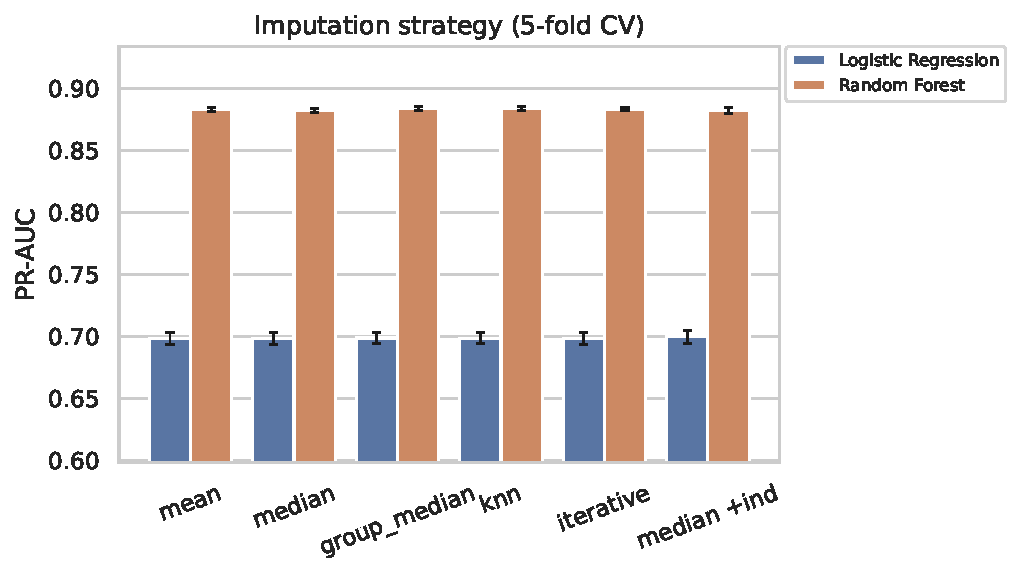
\includegraphics[width=0.9\linewidth]{suite_imputation.pdf}\caption{Imputation.}\label{fig:suite_imputation}\end{figure}
\subsubsection{Scaling}
\begin{table}[H]
\centering
\scriptsize
\begin{adjustbox}{max width=\linewidth}
\begin{tabular}{llrrrrrr}
\toprule
model & scaler & pr\_auc & sd & roc\_auc & f2 & recall & precision \\
\midrule
Logistic Regression & none & 0.6650 & 0.0098 & 0.8449 & 0.6884 & 0.7792 & 0.4696 \\
Logistic Regression & standard & 0.6985 & 0.0045 & 0.8642 & 0.7063 & 0.7801 & 0.5125 \\
Logistic Regression & minmax [0,1] & 0.6996 & 0.0048 & 0.8642 & 0.7066 & 0.7810 & 0.5120 \\
Logistic Regression & minmax [-1,1] & 0.6990 & 0.0049 & 0.8642 & 0.7069 & 0.7808 & 0.5129 \\
Logistic Regression & robust & 0.6986 & 0.0046 & 0.8642 & 0.7060 & 0.7798 & 0.5124 \\
k-NN & none & 0.6153 & 0.0109 & 0.8203 & 0.4926 & 0.4594 & 0.6949 \\
k-NN & standard & 0.7775 & 0.0072 & 0.8827 & 0.6114 & 0.5664 & 0.8964 \\
k-NN & minmax [0,1] & 0.7720 & 0.0072 & 0.8778 & 0.6098 & 0.5646 & 0.8972 \\
k-NN & minmax [-1,1] & 0.7723 & 0.0071 & 0.8779 & 0.6113 & 0.5662 & 0.8975 \\
k-NN & robust & 0.7708 & 0.0070 & 0.8820 & 0.5766 & 0.5288 & 0.9026 \\
SVM (RBF) & standard & 0.8340 & 0.0079 & 0.9075 & 0.7543 & 0.7674 & 0.7063 \\
SVM (RBF) & minmax [0,1] & 0.7966 & 0.0068 & 0.8967 & 0.7365 & 0.7644 & 0.6426 \\
SVM (RBF) & minmax [-1,1] & 0.8040 & 0.0071 & 0.9008 & 0.7433 & 0.7711 & 0.6496 \\
SVM (RBF) & robust & 0.8302 & 0.0082 & 0.9090 & 0.7581 & 0.7768 & 0.6918 \\
\bottomrule
\end{tabular}
\end{adjustbox}
\caption{Scaling methods: 5-fold CV on the training set (F2, recall and precision at threshold 0.5).}
\label{tab:suite_scaling}
\end{table}

\begin{figure}[H]\centering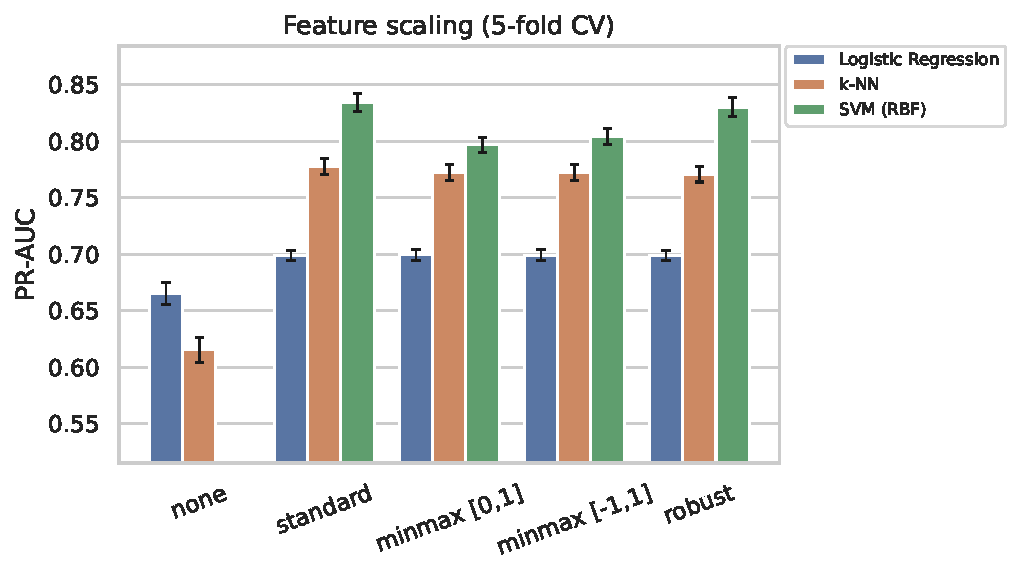
\includegraphics[width=0.9\linewidth]{suite_scaling.pdf}\caption{Scaling.}\label{fig:suite_scaling}\end{figure}
\subsubsection{Outliers and feature engineering}
\begin{table}[H]
\centering
\scriptsize
\begin{adjustbox}{max width=\linewidth}
\begin{tabular}{llrrrrrrr}
\toprule
model & outlier & feat\_eng & pr\_auc & sd & roc\_auc & f2 & recall & precision \\
\midrule
Logistic Regression & none & False & 0.6985 & 0.0045 & 0.8642 & 0.7063 & 0.7801 & 0.5125 \\
Logistic Regression & none & True & 0.7122 & 0.0037 & 0.8761 & 0.7221 & 0.7983 & 0.5226 \\
Logistic Regression & clip\_iqr & False & 0.7021 & 0.0049 & 0.8656 & 0.7082 & 0.7833 & 0.5120 \\
Logistic Regression & clip\_iqr & True & 0.7220 & 0.0053 & 0.8771 & 0.7273 & 0.8022 & 0.5297 \\
Logistic Regression & log & False & 0.7105 & 0.0040 & 0.8717 & 0.7133 & 0.7877 & 0.5179 \\
Logistic Regression & log & True & 0.7160 & 0.0035 & 0.8765 & 0.7227 & 0.7958 & 0.5285 \\
Random Forest & none & False & 0.8827 & 0.0016 & 0.9313 & 0.7685 & 0.7392 & 0.9136 \\
Random Forest & none & True & 0.8852 & 0.0011 & 0.9332 & 0.7721 & 0.7466 & 0.8942 \\
Random Forest & clip\_iqr & False & 0.8834 & 0.0020 & 0.9319 & 0.7690 & 0.7396 & 0.9146 \\
Random Forest & clip\_iqr & True & 0.8854 & 0.0011 & 0.9333 & 0.7718 & 0.7461 & 0.8951 \\
Random Forest & log & False & 0.8825 & 0.0018 & 0.9312 & 0.7685 & 0.7390 & 0.9143 \\
Random Forest & log & True & 0.8852 & 0.0011 & 0.9331 & 0.7721 & 0.7466 & 0.8942 \\
\bottomrule
\end{tabular}
\end{adjustbox}
\caption{Outlier handling and feature engineering: 5-fold CV on the training set (F2, recall and precision at threshold 0.5).}
\label{tab:suite_outlier_fe}
\end{table}

\begin{figure}[H]\centering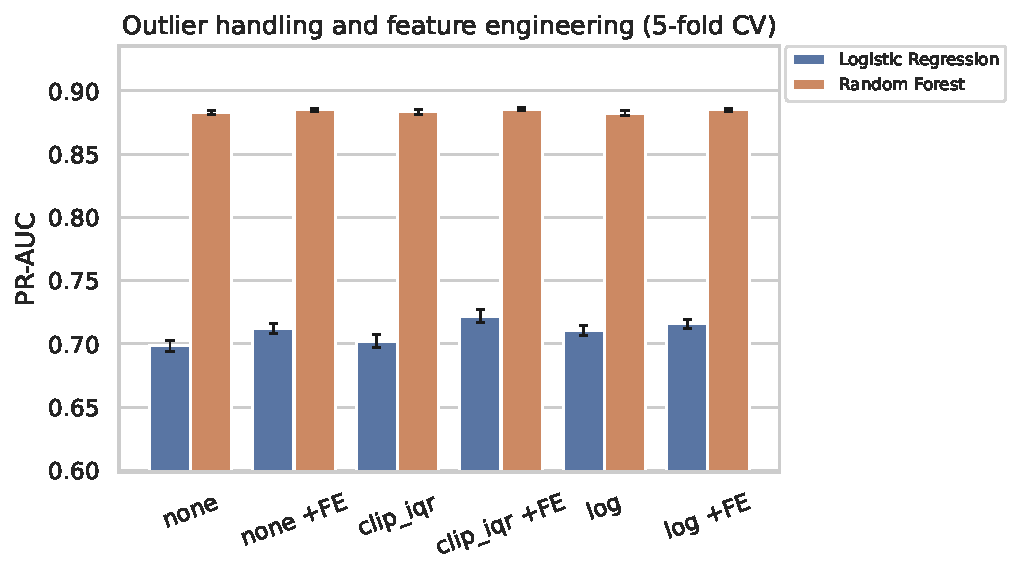
\includegraphics[width=0.9\linewidth]{suite_outlier_fe.pdf}\caption{Outliers.}\label{fig:suite_outlier_fe}\end{figure}
\subsubsection{Encoding}
\begin{table}[H]
\centering
\scriptsize
\begin{adjustbox}{max width=\linewidth}
\begin{tabular}{llrrrrrr}
\toprule
model & grade\_encoding & pr\_auc & sd & roc\_auc & f2 & recall & precision \\
\midrule
Logistic Regression & ordinal & 0.6985 & 0.0045 & 0.8642 & 0.7063 & 0.7801 & 0.5125 \\
Logistic Regression & onehot & 0.7165 & 0.0061 & 0.8708 & 0.7181 & 0.7791 & 0.5470 \\
k-NN & ordinal & 0.7775 & 0.0072 & 0.8827 & 0.6114 & 0.5664 & 0.8964 \\
k-NN & onehot & 0.7748 & 0.0083 & 0.8787 & 0.6179 & 0.5743 & 0.8871 \\
Random Forest & ordinal & 0.8827 & 0.0016 & 0.9313 & 0.7685 & 0.7392 & 0.9136 \\
Random Forest & onehot & 0.8819 & 0.0018 & 0.9309 & 0.7667 & 0.7392 & 0.9010 \\
\bottomrule
\end{tabular}
\end{adjustbox}
\caption{Encoding of the loan grade: 5-fold CV on the training set (F2, recall and precision at threshold 0.5).}
\label{tab:suite_encoding}
\end{table}

\subsubsection{Dimensionality}
\begin{table}[H]
\centering
\scriptsize
\begin{adjustbox}{max width=\linewidth}
\begin{tabular}{llrrrrrr}
\toprule
model & reduction & pr\_auc & sd & roc\_auc & f2 & recall & precision \\
\midrule
Logistic Regression & none & 0.6985 & 0.0045 & 0.8642 & 0.7063 & 0.7801 & 0.5125 \\
Logistic Regression & PCA 80\% & 0.6485 & 0.0095 & 0.8391 & 0.6867 & 0.7755 & 0.4711 \\
Logistic Regression & PCA 90\% & 0.6571 & 0.0048 & 0.8447 & 0.6869 & 0.7685 & 0.4824 \\
Logistic Regression & PCA 95\% & 0.6755 & 0.0086 & 0.8517 & 0.6957 & 0.7764 & 0.4915 \\
Logistic Regression & PCA 99\% & 0.6983 & 0.0046 & 0.8642 & 0.7064 & 0.7805 & 0.5123 \\
Logistic Regression & SelectKBest k=5 & 0.6693 & 0.0055 & 0.8475 & 0.6984 & 0.7798 & 0.4927 \\
Logistic Regression & SelectKBest k=10 & 0.6837 & 0.0053 & 0.8572 & 0.7007 & 0.7745 & 0.5075 \\
Logistic Regression & SelectKBest k=15 & 0.6920 & 0.0059 & 0.8614 & 0.7009 & 0.7739 & 0.5090 \\
k-NN & none & 0.7775 & 0.0072 & 0.8827 & 0.6114 & 0.5664 & 0.8964 \\
k-NN & PCA 80\% & 0.7251 & 0.0217 & 0.8648 & 0.5695 & 0.5317 & 0.7960 \\
k-NN & PCA 90\% & 0.7462 & 0.0092 & 0.8732 & 0.5939 & 0.5544 & 0.8304 \\
k-NN & PCA 95\% & 0.7550 & 0.0099 & 0.8755 & 0.5954 & 0.5528 & 0.8610 \\
k-NN & PCA 99\% & 0.7776 & 0.0070 & 0.8827 & 0.6112 & 0.5662 & 0.8958 \\
k-NN & SelectKBest k=5 & 0.7592 & 0.0045 & 0.8731 & 0.6281 & 0.5943 & 0.8136 \\
k-NN & SelectKBest k=10 & 0.7695 & 0.0077 & 0.8841 & 0.6429 & 0.6105 & 0.8170 \\
k-NN & SelectKBest k=15 & 0.7823 & 0.0110 & 0.8851 & 0.6258 & 0.5828 & 0.8890 \\
Random Forest & none & 0.8826 & 0.0017 & 0.9313 & 0.7677 & 0.7383 & 0.9133 \\
Random Forest & PCA 80\% & 0.7664 & 0.0296 & 0.8822 & 0.6810 & 0.6794 & 0.6880 \\
Random Forest & PCA 90\% & 0.8196 & 0.0074 & 0.9041 & 0.7096 & 0.6978 & 0.7612 \\
Random Forest & PCA 95\% & 0.8280 & 0.0073 & 0.9072 & 0.7148 & 0.7002 & 0.7800 \\
Random Forest & PCA 99\% & 0.8363 & 0.0076 & 0.9100 & 0.7300 & 0.7156 & 0.7945 \\
Random Forest & SelectKBest k=5 & 0.8301 & 0.0047 & 0.9053 & 0.7376 & 0.7374 & 0.7385 \\
Random Forest & SelectKBest k=10 & 0.8355 & 0.0068 & 0.9122 & 0.7463 & 0.7491 & 0.7359 \\
Random Forest & SelectKBest k=15 & 0.8684 & 0.0045 & 0.9253 & 0.7553 & 0.7369 & 0.8400 \\
\bottomrule
\end{tabular}
\end{adjustbox}
\caption{PCA and univariate feature selection: 5-fold CV on the training set (F2, recall and precision at threshold 0.5).}
\label{tab:suite_dimensionality}
\end{table}

\begin{figure}[H]\centering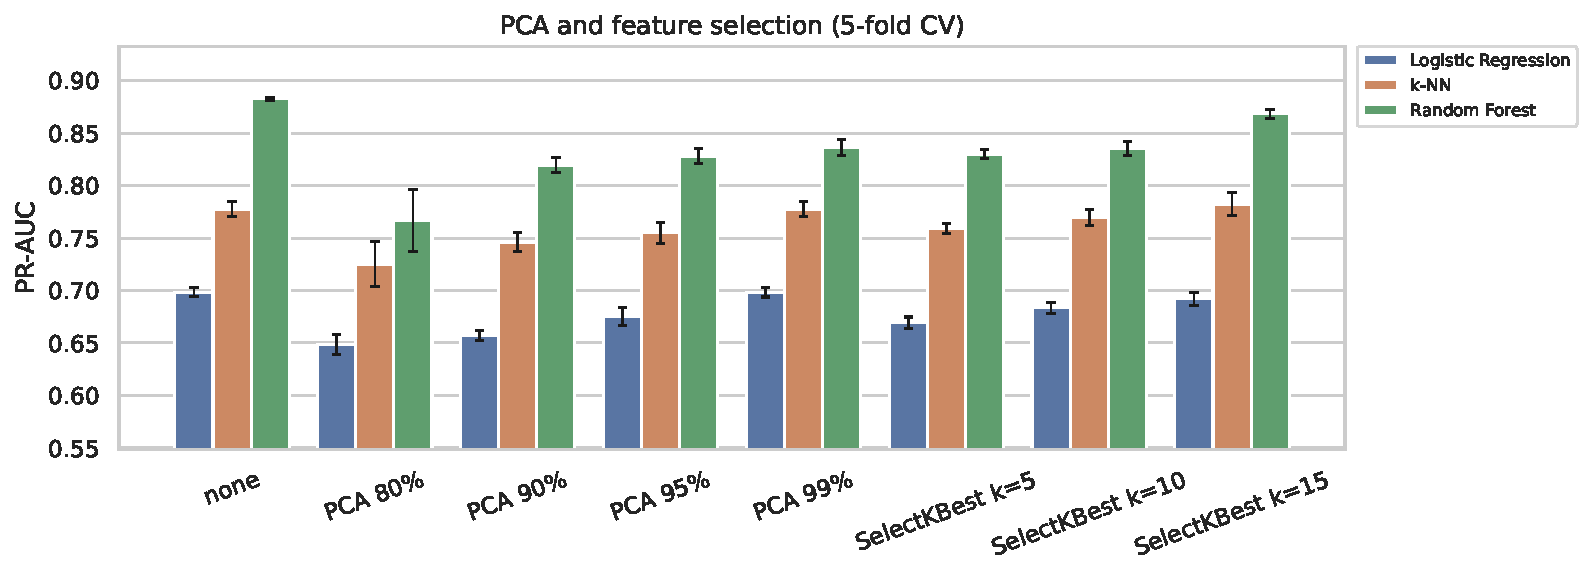
\includegraphics[width=0.9\linewidth]{suite_dimensionality.pdf}\caption{Dimensionality.}\label{fig:suite_dimensionality}\end{figure}
\subsubsection{Imbalance}
\begin{table}[H]
\centering
\scriptsize
\begin{adjustbox}{max width=\linewidth}
\begin{tabular}{llrrrrrr}
\toprule
model & imbalance & pr\_auc & sd & roc\_auc & f2 & recall & precision \\
\midrule
Logistic Regression & none & 0.7026 & 0.0039 & 0.8637 & 0.5390 & 0.5050 & 0.7381 \\
Logistic Regression & class\_weight & 0.6985 & 0.0045 & 0.8642 & 0.7063 & 0.7801 & 0.5125 \\
Logistic Regression & smote & 0.6983 & 0.0050 & 0.8638 & 0.7041 & 0.7750 & 0.5155 \\
Logistic Regression & undersample & 0.6983 & 0.0038 & 0.8641 & 0.7080 & 0.7822 & 0.5133 \\
Random Forest & none & 0.8843 & 0.0017 & 0.9314 & 0.7554 & 0.7152 & 0.9743 \\
Random Forest & class\_weight & 0.8827 & 0.0016 & 0.9313 & 0.7685 & 0.7392 & 0.9136 \\
Random Forest & smote & 0.8792 & 0.0023 & 0.9280 & 0.7568 & 0.7182 & 0.9641 \\
Random Forest & undersample & 0.8766 & 0.0016 & 0.9291 & 0.7809 & 0.7939 & 0.7334 \\
Hist. Gradient Boosting & none & 0.8982 & 0.0016 & 0.9440 & 0.7657 & 0.7265 & 0.9761 \\
Hist. Gradient Boosting & class\_weight & 0.8986 & 0.0029 & 0.9442 & 0.7923 & 0.7819 & 0.8370 \\
Hist. Gradient Boosting & smote & 0.8974 & 0.0016 & 0.9428 & 0.7678 & 0.7288 & 0.9766 \\
Hist. Gradient Boosting & undersample & 0.8928 & 0.0023 & 0.9406 & 0.7921 & 0.7962 & 0.7762 \\
\bottomrule
\end{tabular}
\end{adjustbox}
\caption{Class-imbalance strategies: 5-fold CV on the training set (F2, recall and precision at threshold 0.5).}
\label{tab:suite_imbalance}
\end{table}

\begin{figure}[H]\centering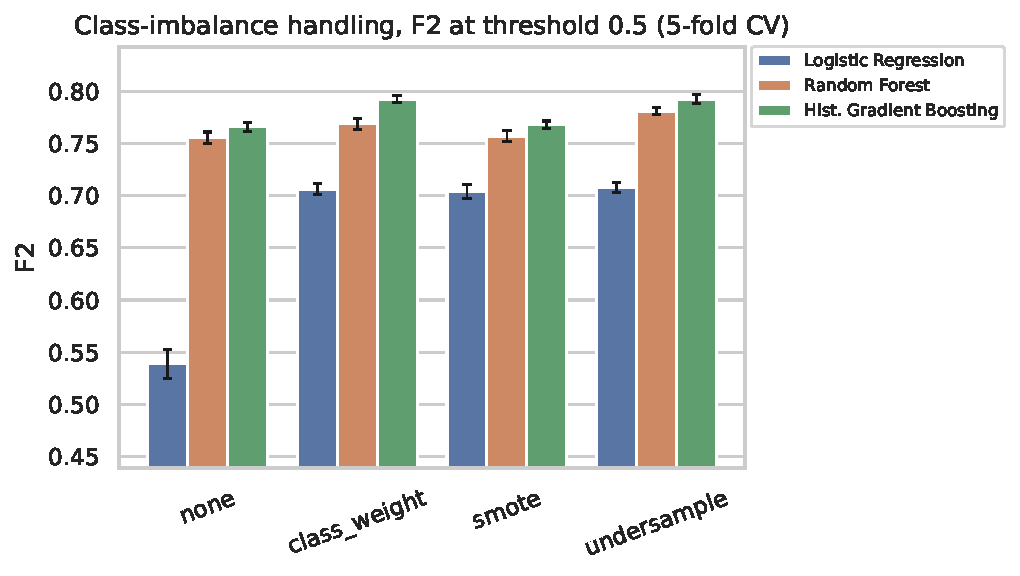
\includegraphics[width=0.9\linewidth]{suite_imbalance.pdf}\caption{Imbalance.}\label{fig:suite_imbalance}\end{figure}

\subsection{Tuned models}
\begin{table}[H]
\centering
\scriptsize
\begin{adjustbox}{max width=\linewidth}
\begin{tabular}{lp{5.4cm}rrrrr}
\toprule
model & best\_params & CV PR-AUC & sd & CV ROC-AUC & CV F2 & time (s) \\
\midrule
Logistic Regression & C=10, class\_weight=None & 0.7538 & 0.0072 & 0.8827 & 0.6247 & 3.6 \\
Linear SVM & C=1, class\_weight=None & 0.7473 & 0.0071 & 0.8801 & 0.6152 & 2.4 \\
SVM (RBF) & C=10, gamma=scale & 0.8501 & 0.0045 & 0.9115 & 0.7634 & 164.5 \\
k-NN & n\_neighbors=15, weights=distance & 0.8134 & 0.0058 & 0.8934 & 0.6459 & 12.5 \\
Gaussian Naive Bayes & var\_smoothing=0.001 & 0.6229 & 0.0120 & 0.8552 & 0.6077 & 0.9 \\
Decision Tree & class\_weight=None, max\_depth=10, min\_samples\_leaf=20 & 0.8598 & 0.0040 & 0.9151 & 0.7438 & 5.6 \\
Random Forest & class\_weight=None, max\_features=0.5, min\_samples\_leaf=3 & 0.8902 & 0.0025 & 0.9341 & 0.7526 & 198.4 \\
Hist. Gradient Boosting & class\_weight=None, learning\_rate=0.05, max\_iter=300, max\_leaf\_nodes=31 & 0.8988 & 0.0026 & 0.9441 & 0.7656 & 22.1 \\
\bottomrule
\end{tabular}
\end{adjustbox}
\caption{Grid-search results (5-fold CV, refit on PR-AUC; F2 at threshold 0.5).}
\label{tab:tuning}
\end{table}

\begin{table}[H]
\centering
\small
\begin{adjustbox}{max width=\linewidth}
\begin{tabular}{lrrrrrrr}
\toprule
model & pr\_auc & roc\_auc & threshold & F2 & recall & precision & accuracy \\
\midrule
Hist. Gradient Boosting & \textbf{0.9045} & \textbf{0.9459} & 0.1515 & \textbf{0.8132} & \textbf{0.8512} & 0.6901 & 0.8839 \\
Random Forest & 0.8934 & 0.9361 & 0.2222 & 0.8021 & 0.8068 & 0.7841 & 0.9092 \\
Decision Tree & 0.8623 & 0.9180 & 0.1414 & 0.7670 & 0.7856 & 0.7006 & 0.8797 \\
SVM (RBF) & 0.8561 & 0.9147 & -0.4900 & 0.7703 & 0.8117 & 0.6398 & 0.8589 \\
k-NN & 0.8163 & 0.8925 & 0.2424 & 0.7501 & 0.7906 & 0.6228 & 0.8495 \\
Logistic Regression & 0.7512 & 0.8797 & 0.2224 & 0.7360 & 0.7955 & 0.5665 & 0.8222 \\
Linear SVM & 0.7443 & 0.8774 & -0.4521 & 0.7339 & 0.7962 & 0.5589 & 0.8180 \\
Gaussian Naive Bayes & 0.6244 & 0.8503 & 0.0101 & 0.7140 & 0.8096 & 0.4850 & 0.7704 \\
\bottomrule
\end{tabular}
\end{adjustbox}
\caption{Test-set results of the tuned traditional models; F2, recall, precision and accuracy at the F2-tuned threshold.}
\label{tab:test_traditional}
\end{table}

\begin{figure}[H]\centering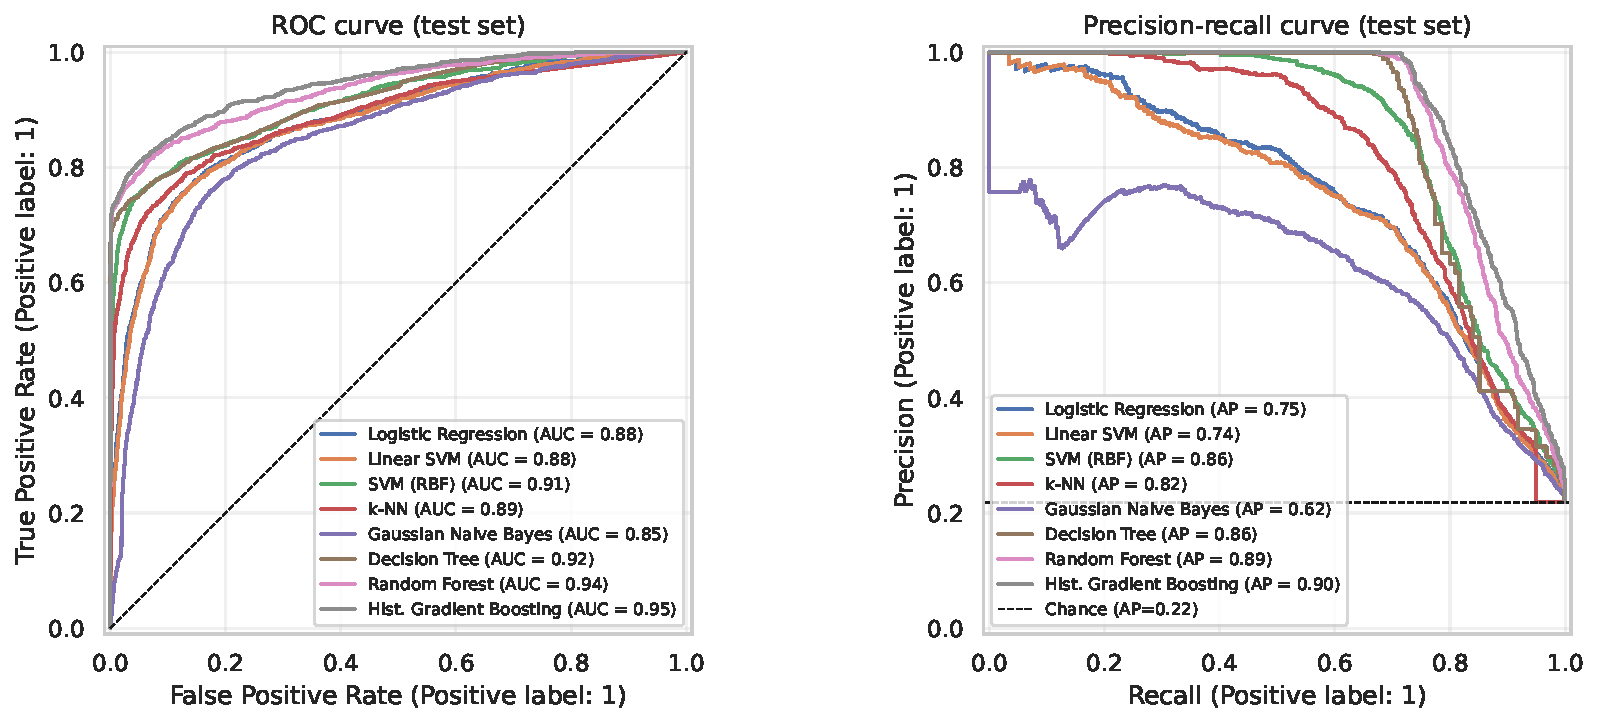
\includegraphics[width=\linewidth]{roc_pr_traditional.pdf}\caption{ROC.}\label{fig:roc_trad}\end{figure}
\begin{figure}[H]\centering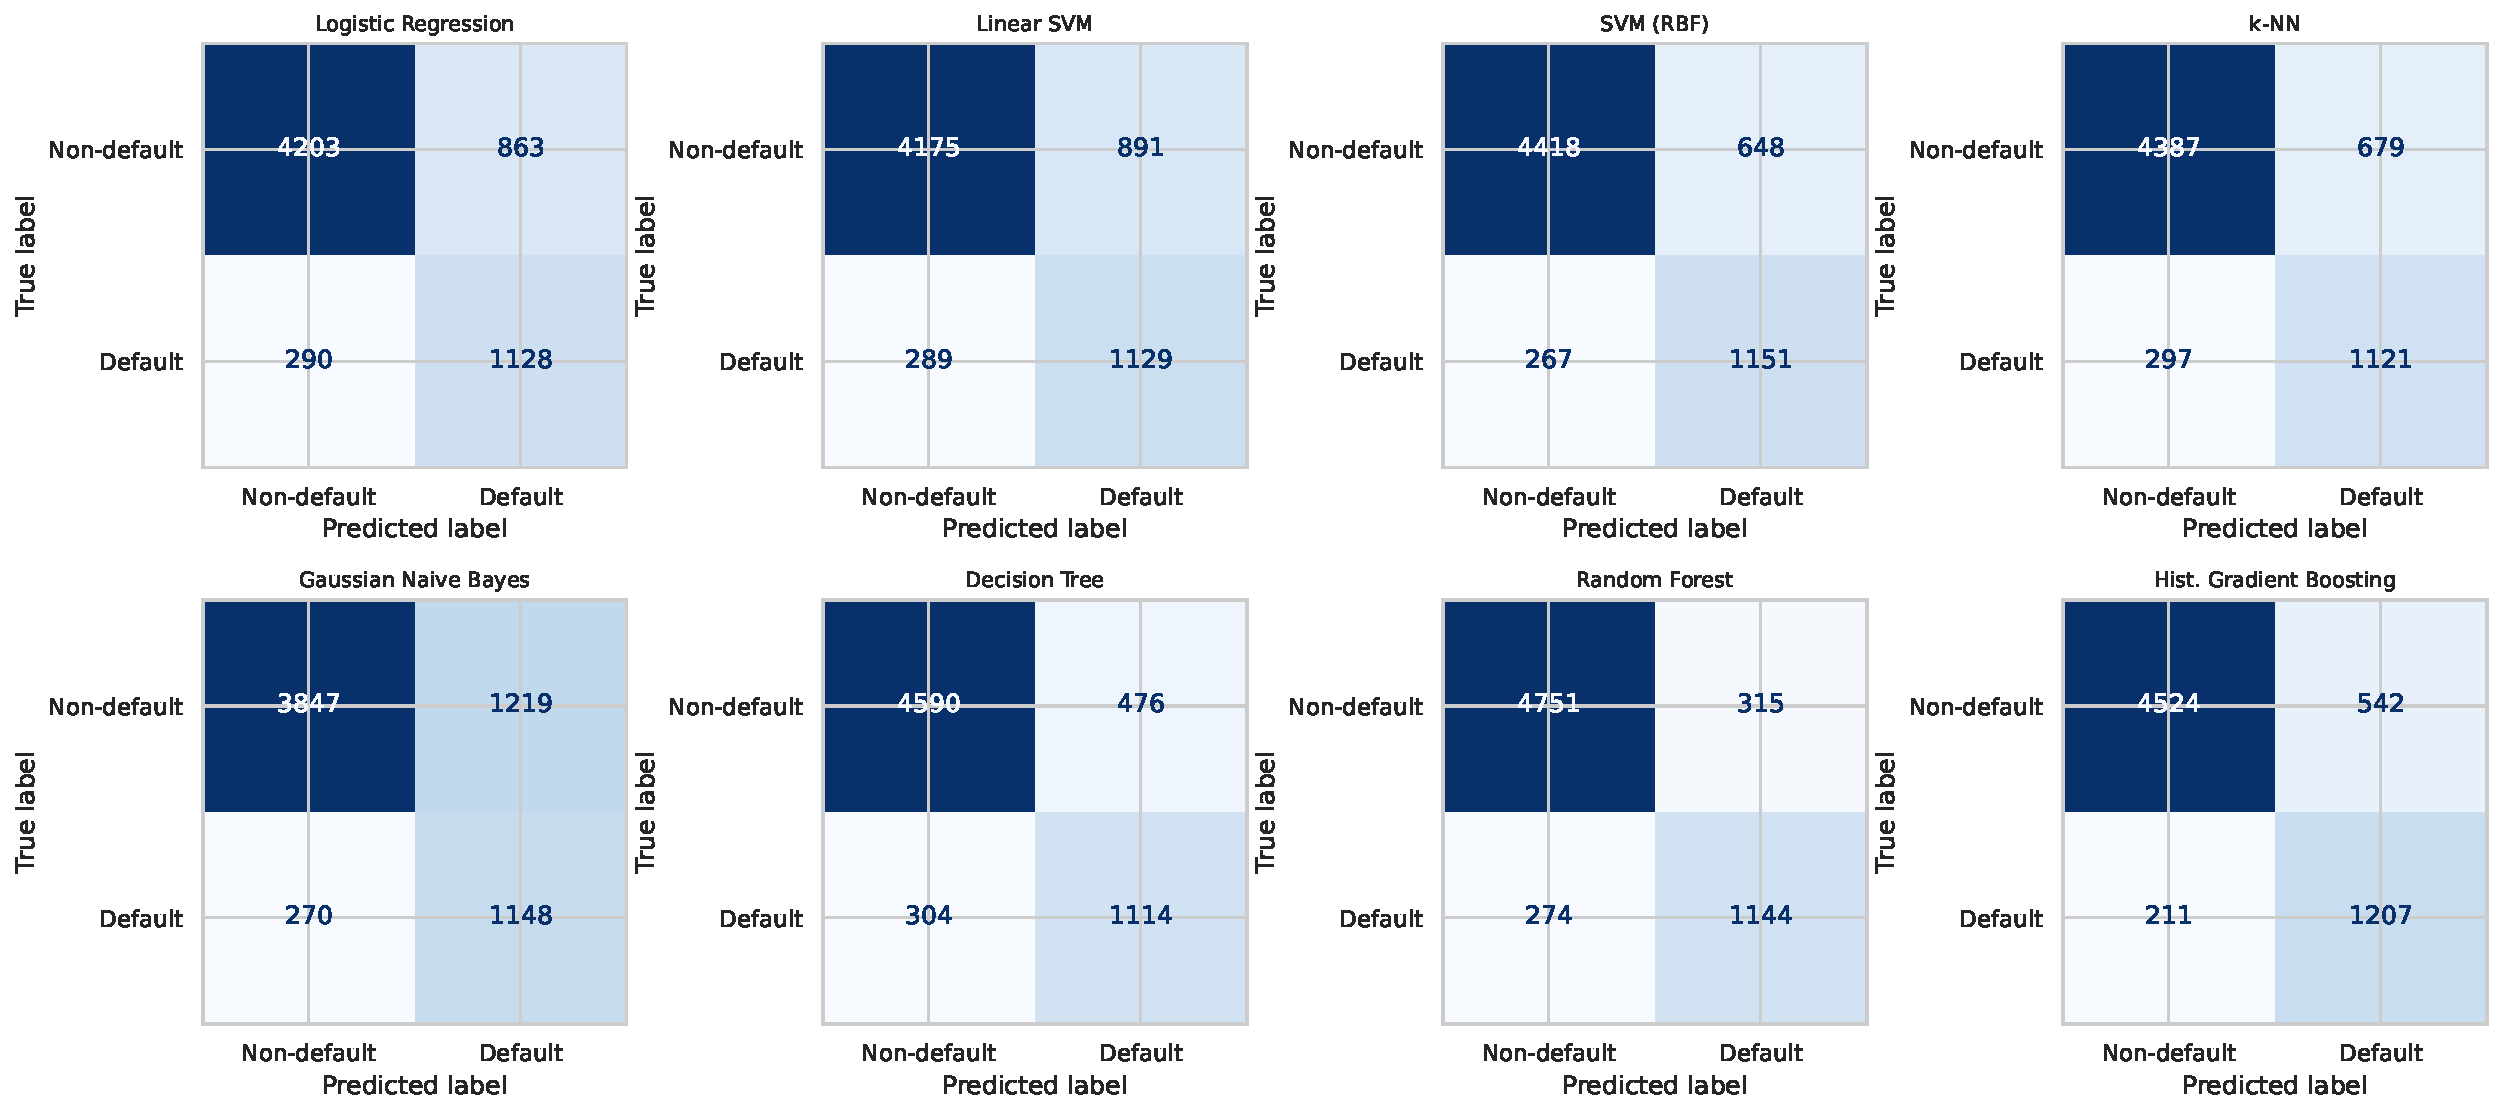
\includegraphics[width=\linewidth]{confusion_traditional.pdf}\caption{Confusion.}\label{fig:confusion}\end{figure}
\begin{figure}[H]\centering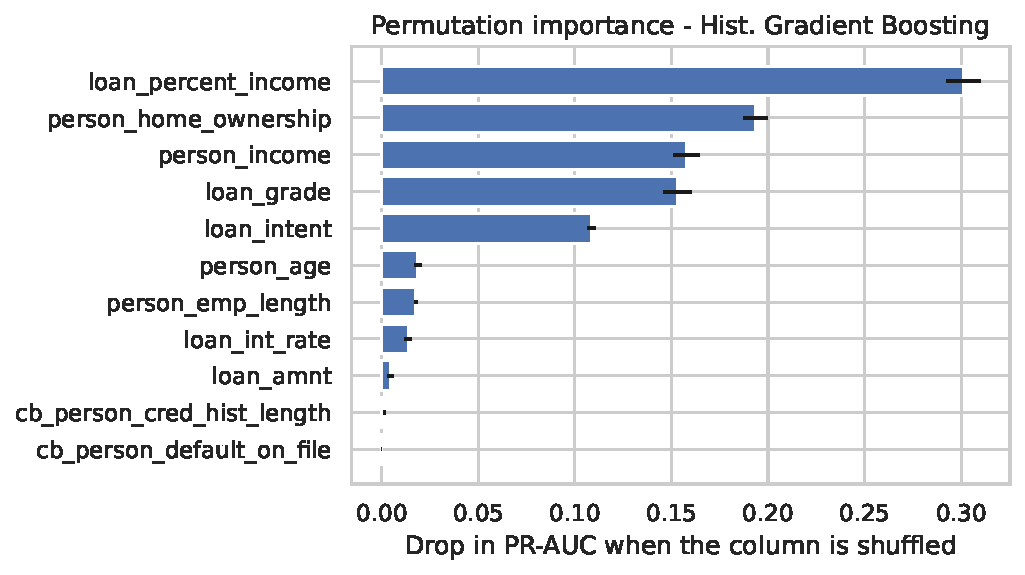
\includegraphics[width=0.7\linewidth]{importance_best.pdf}\caption{Importance.}\label{fig:importance}\end{figure}

\subsection{Deep learning}
\begin{table}[H]
\centering
\scriptsize
\begin{adjustbox}{max width=\linewidth}
\begin{tabular}{lrrrrrrr}
\toprule
model & val PR-AUC & pr\_auc & roc\_auc & F2 & recall & epochs & time (s) \\
\midrule
MLP 128-64 (reference) & 0.8729 & 0.8640 & 0.9221 & 0.7616 & 0.7955 & 69 & 9.9 \\
MLP 64-32 (smaller) & 0.8693 & 0.8633 & 0.9223 & 0.7623 & 0.7743 & 63 & 6.0 \\
MLP 256-128-64 (deeper) & 0.8724 & 0.8658 & 0.9226 & 0.7651 & 0.7913 & 40 & 9.7 \\
No dropout & 0.8662 & 0.8619 & 0.9213 & 0.7659 & 0.7948 & 49 & 3.8 \\
One-hot instead of embeddings & 0.8709 & 0.8647 & 0.9214 & 0.7634 & 0.7736 & 81 & 8.4 \\
No class weighting & 0.8712 & 0.8633 & 0.9201 & 0.7572 & 0.7898 & 47 & 5.1 \\
No engineered features & 0.8671 & 0.8605 & 0.9196 & 0.7627 & 0.8004 & 39 & 4.2 \\
\bottomrule
\end{tabular}
\end{adjustbox}
\caption{MLP variants: validation PR-AUC (used for selection) and test metrics.}
\label{tab:mlp}
\end{table}

\begin{table}[H]
\centering
\small
\begin{adjustbox}{max width=\linewidth}
\begin{tabular}{lrrrrrrr}
\toprule
model & pr\_auc & roc\_auc & F2 & recall & precision & accuracy & time (s) \\
\midrule
MLP 128-64 (reference) & 0.8619 $\pm$ 0.0017 & 0.9200 $\pm$ 0.0017 & 0.7621 $\pm$ 0.0017 & 0.7956 $\pm$ 0.0088 & 0.6535 $\pm$ 0.0283 & 0.8626 $\pm$ 0.0105 & 6.8 \\
TabNet & 0.8612 $\pm$ 0.0026 & 0.9180 $\pm$ 0.0014 & 0.7568 $\pm$ 0.0039 & 0.7984 $\pm$ 0.0170 & 0.6288 $\pm$ 0.0398 & 0.8517 $\pm$ 0.0148 & 34.0 \\
\bottomrule
\end{tabular}
\end{adjustbox}
\caption{Deep learning models on the test set, mean $\pm$ sd over 5 seeds (threshold tuned for F2 on a validation split; training time per seed).}
\label{tab:deep}
\end{table}

\begin{figure}[H]\centering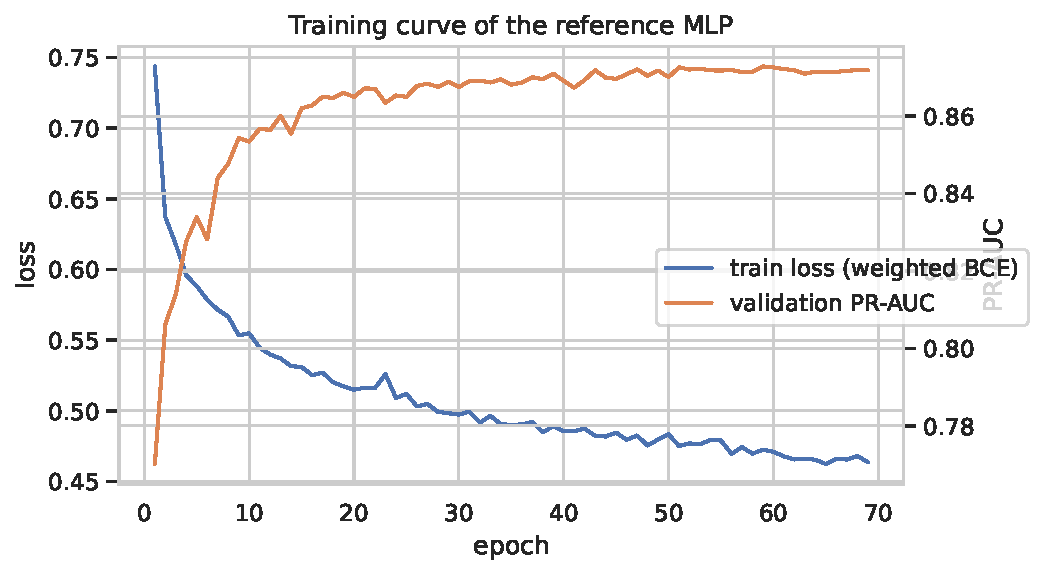
\includegraphics[width=0.6\linewidth]{mlp_training.pdf}\caption{MLP.}\label{fig:mlp_training}\end{figure}
\begin{figure}[H]\centering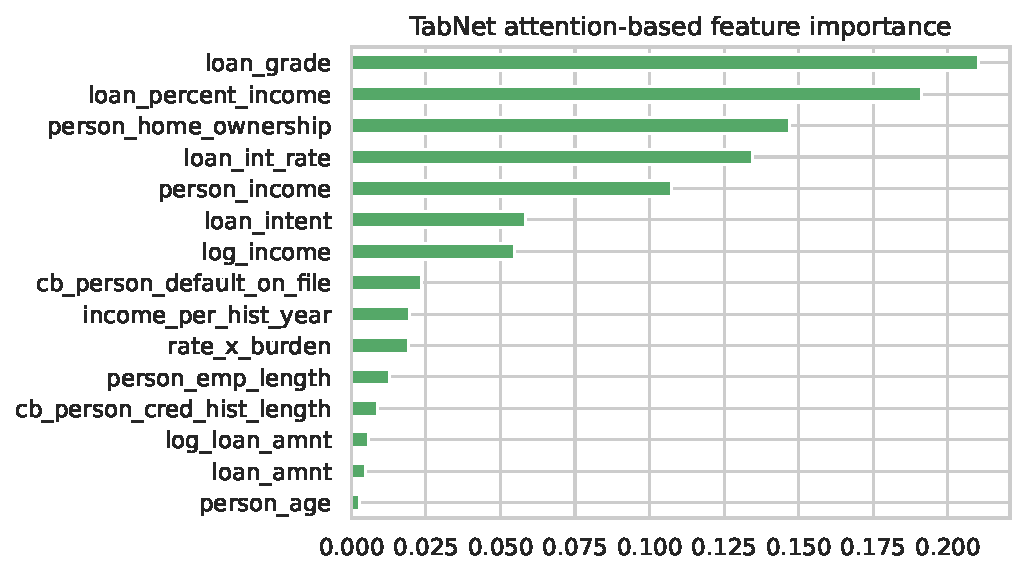
\includegraphics[width=0.6\linewidth]{tabnet_importance.pdf}\caption{TabNet.}\label{fig:tabnet}\end{figure}
\begin{figure}[H]\centering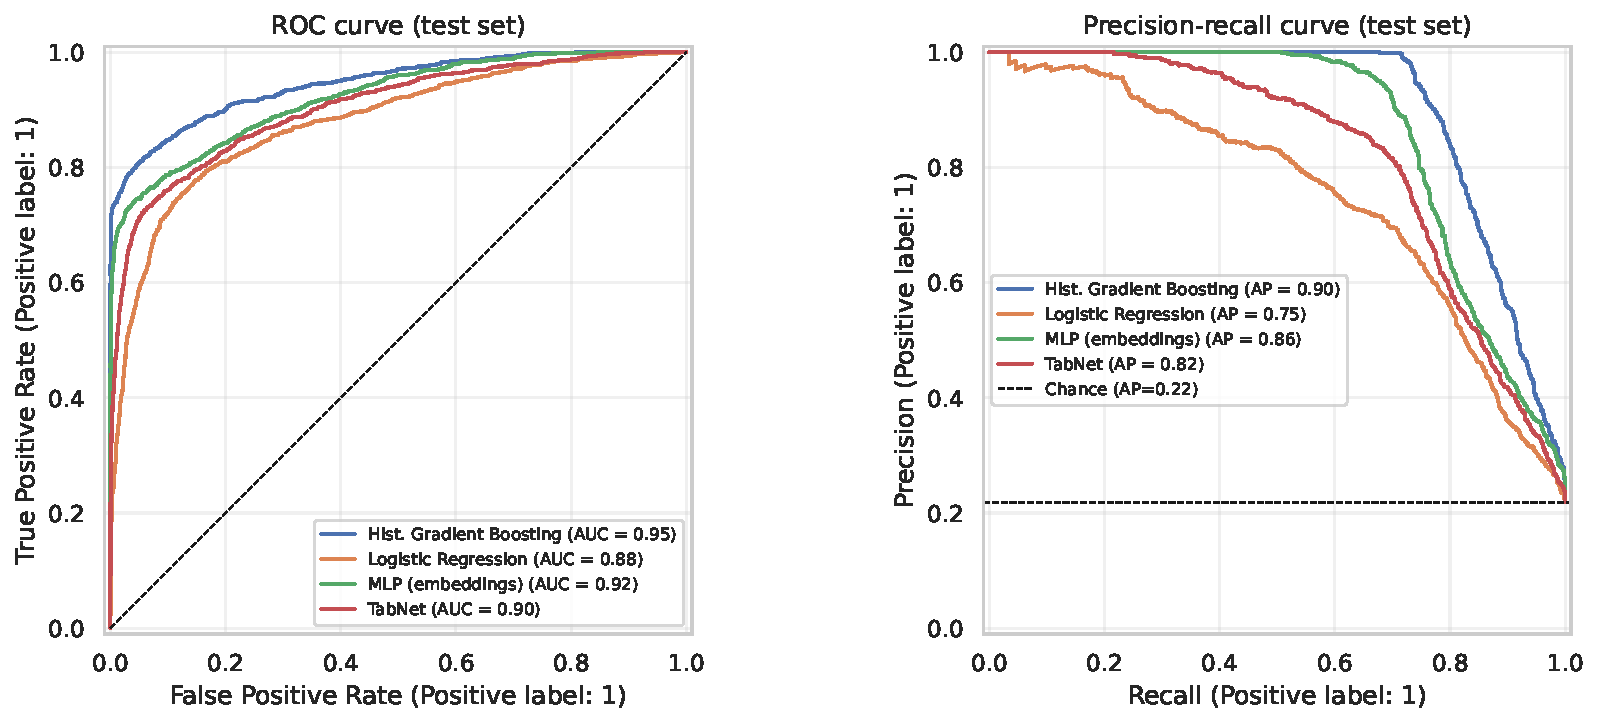
\includegraphics[width=\linewidth]{roc_pr_traditional_vs_deep.pdf}\caption{Trad vs deep.}\label{fig:roc_deep}\end{figure}

\subsection{Bayesian network}
\begin{table}[H]
\centering
\small
\begin{adjustbox}{max width=\linewidth}
\begin{tabular}{rrrrrr}
\toprule
n\_bins & alpha & Expert DAG & Hill-climb BIC & Naive Bayes & TAN \\
\midrule
3 & 0.1 & 0.7024 & 0.6088 & 0.6251 & 0.7401 \\
3 & 1 & 0.7015 & 0.6111 & 0.6249 & 0.7393 \\
3 & 10 & 0.6912 & 0.6114 & 0.6261 & 0.7312 \\
5 & 0.1 & 0.7338 & 0.6479 & 0.6633 & 0.7672 \\
5 & 1 & 0.7316 & 0.6479 & 0.6649 & 0.7656 \\
5 & 10 & 0.7111 & 0.6457 & 0.6645 & 0.7578 \\
8 & 0.1 & 0.7948 & 0.6859 & 0.6905 & 0.7915 \\
8 & 1 & 0.7908 & 0.6879 & 0.6919 & 0.7893 \\
8 & 10 & 0.7674 & 0.6871 & 0.6916 & 0.7787 \\
12 & 0.1 & 0.7940 & 0.7416 & 0.6940 & 0.7542 \\
12 & 1 & 0.7915 & 0.7416 & 0.6956 & 0.7515 \\
12 & 10 & 0.7780 & 0.7383 & 0.6954 & 0.7403 \\
\bottomrule
\end{tabular}
\end{adjustbox}
\caption{Bayesian networks: validation PR-AUC by number of bins and Dirichlet pseudo-count $\alpha$.}
\label{tab:bn_sens}
\end{table}

\begin{table}[H]
\centering
\scriptsize
\begin{adjustbox}{max width=\linewidth}
\begin{tabular}{lrrrrrrrrrrr}
\toprule
structure & bins & alpha & edges & parameters & test log-lik. & pr\_auc & roc\_auc & F2 & recall & precision & accuracy \\
\midrule
Expert DAG & 8 & 0.1 & 12 & 2041 & -100750 & 0.7822 & 0.8712 & 0.7152 & 0.7736 & 0.5493 & 0.8117 \\
Hill-climb BIC & 12 & 0.1 & 17 & 3736 & -103692 & 0.7332 & 0.8579 & 0.7033 & 0.7941 & 0.4826 & 0.7688 \\
Naive Bayes & 12 & 1 & 11 & 171 & -136946 & 0.7061 & 0.8635 & 0.7149 & 0.7962 & 0.5076 & 0.7866 \\
TAN & 8 & 0.1 & 21 & 777 & -105532 & \textbf{0.7895} & \textbf{0.8900} & 0.7390 & 0.8110 & 0.5453 & 0.8108 \\
\bottomrule
\end{tabular}
\end{adjustbox}
\caption{Bayesian-network structures on the test set, each with the bins and $\alpha$ selected on validation data.}
\label{tab:bn_results}
\end{table}

\begin{figure}[H]\centering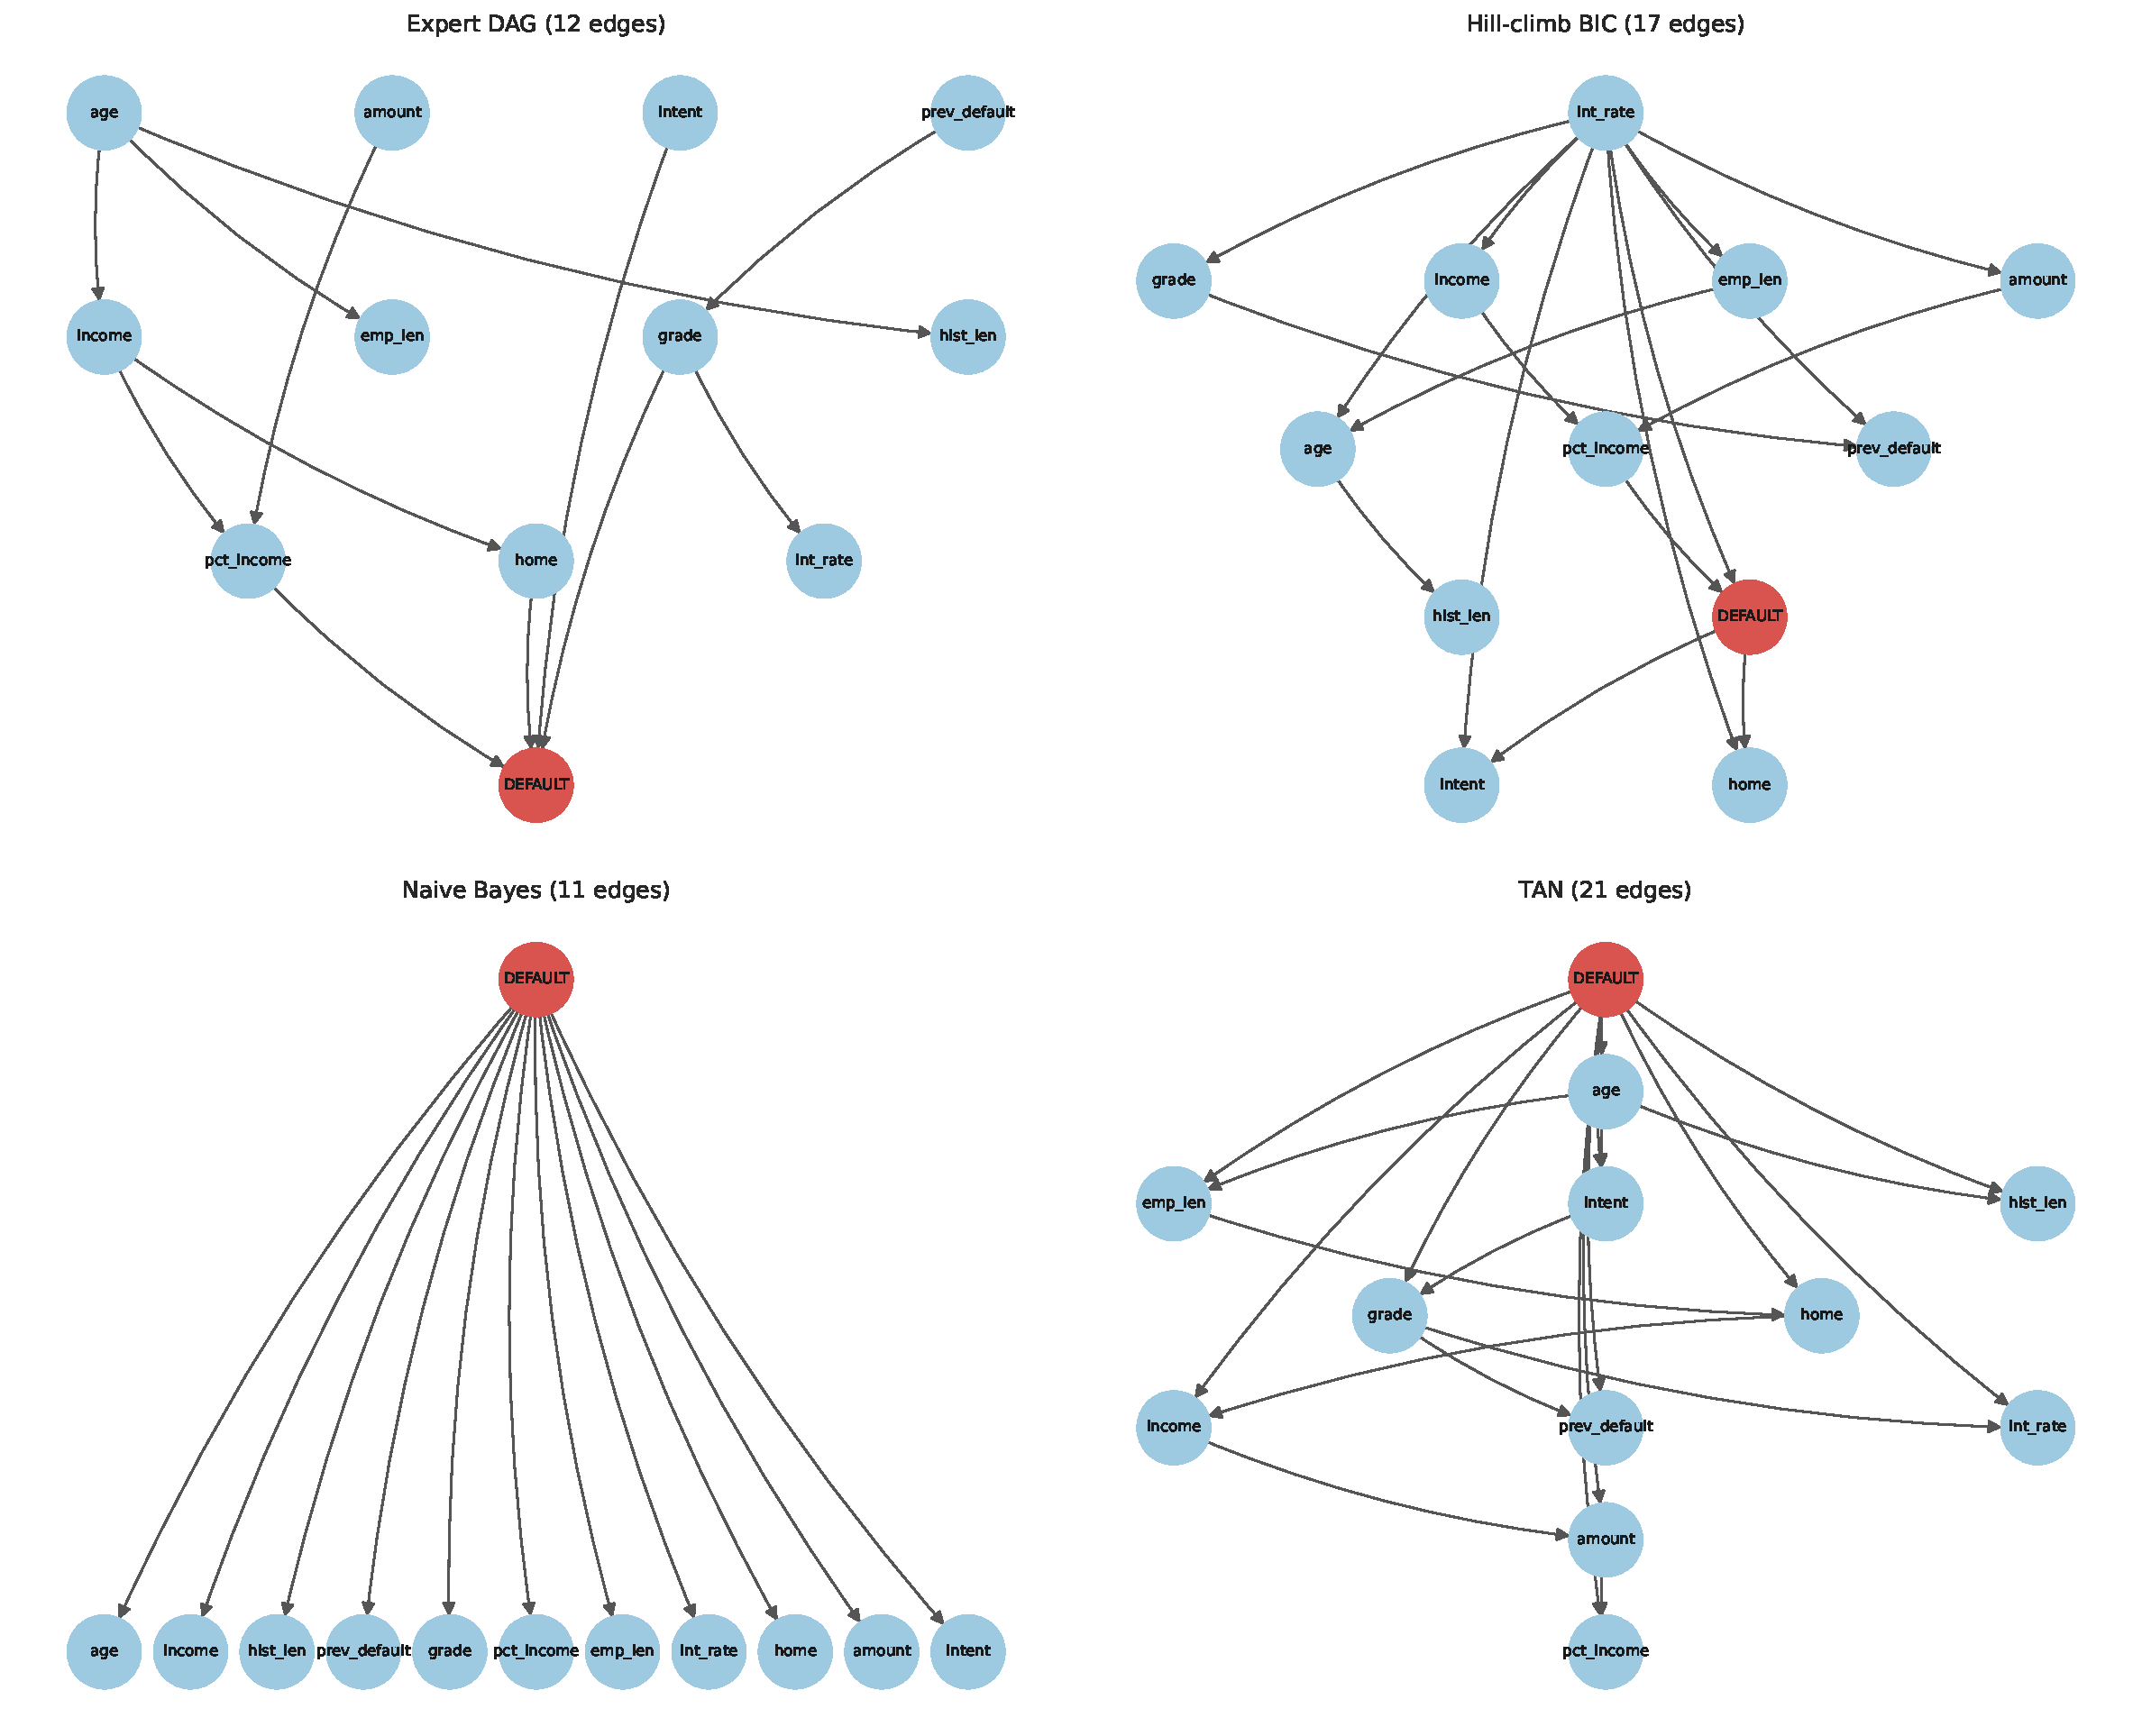
\includegraphics[width=\linewidth]{bn_structures.pdf}\caption{Structures.}\label{fig:bn_structures}\end{figure}
\begin{figure}[H]\centering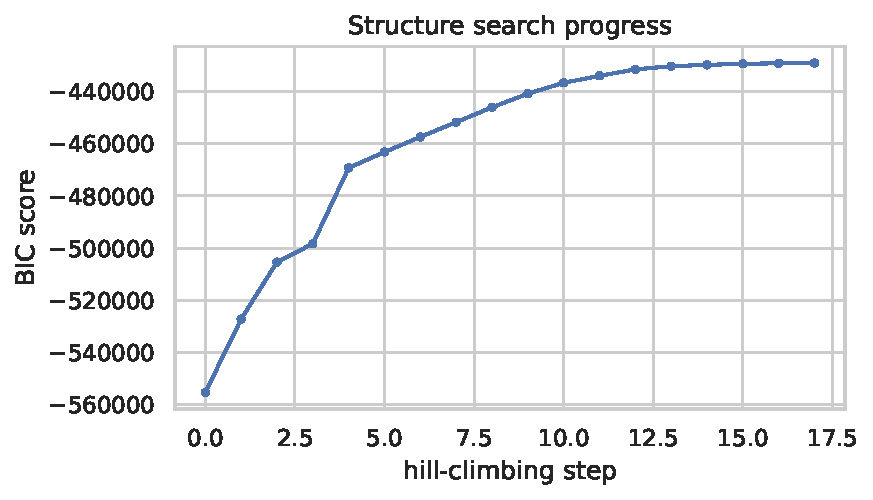
\includegraphics[width=0.6\linewidth]{bn_bic_trace.pdf}\caption{BIC.}\label{fig:bic}\end{figure}
\begin{table}[H]
\centering
\small
\begin{adjustbox}{max width=\linewidth}
\begin{tabular}{lrrrr}
\toprule
query & empirical & support & TAN & Expert DAG \\
\midrule
P(default) & 0.2187 & 25932 & 0.2187 & 0.2594 \\
P(default \textbar{} grade=A) & 0.0998 & 8584 & 0.0998 & 0.1750 \\
P(default \textbar{} grade=D) & 0.5902 & 2889 & 0.5900 & 0.5749 \\
P(default \textbar{} grade=G) & 0.9792 & 48 & 0.9675 & 0.6361 \\
P(default \textbar{} home=RENT) & 0.3167 & 13114 & 0.3149 & 0.3675 \\
P(default \textbar{} home=OWN) & 0.0715 & 2042 & 0.0681 & 0.1696 \\
P(default \textbar{} grade=D, home=OWN) & 0.0463 & 216 & 0.2731 & 0.0780 \\
P(default \textbar{} intent=MEDICAL) & 0.2672 & 4842 & 0.2672 & 0.3008 \\
P(default \textbar{} intent=VENTURE) & 0.1505 & 4610 & 0.1506 & 0.1901 \\
P(prev\_default=Y \textbar{} default=1) & 0.3063 & 5671 & 0.3064 & 0.2685 \\
P(prev\_default=Y \textbar{} default=0) & 0.1404 & 20261 & 0.1404 & 0.1445 \\
P(grade in D..G \textbar{} default=1) & 0.4195 & 5671 & 0.4196 & 0.3408 \\
P(grade in D..G \textbar{} default=0) & 0.0746 & 20261 & 0.0747 & 0.0832 \\
\bottomrule
\end{tabular}
\end{adjustbox}
\caption{Exact answers of two networks (variable elimination) against the empirical frequency in the training data; support is the number of training rows matching the evidence.}
\label{tab:bn_queries}
\end{table}

\begin{table}[H]
\centering
\small
\begin{adjustbox}{max width=\linewidth}
\begin{tabular}{lrrrr}
\toprule
method & samples & MAE, 2 evid. & MAE, 5 evid. & MAE, 10 evid. \\
\midrule
Gibbs sampling & 100 & 0.0444 & 0.0353 & 0.0159 \\
Gibbs sampling & 1000 & 0.0154 & 0.0124 & 0.0057 \\
Gibbs sampling & 10000 & 0.0061 & 0.0043 & 0.0025 \\
Likelihood weighting & 100 & 0.0467 & 0.0356 & 0.0183 \\
Likelihood weighting & 1000 & 0.0160 & 0.0131 & 0.0057 \\
Likelihood weighting & 10000 & 0.0049 & 0.0030 & 0.0015 \\
Rejection sampling & 100 & 0.1636 & 0.3041 & 0.3868 \\
Rejection sampling & 1000 & 0.0639 & 0.2514 & 0.3868 \\
Rejection sampling & 10000 & 0.0178 & 0.1673 & 0.3788 \\
\bottomrule
\end{tabular}
\end{adjustbox}
\caption{Mean absolute error of approximate $P(\text{default} \mid \bm{e})$ against variable elimination (60 random test applicants per evidence size).}
\label{tab:bn_inference}
\end{table}

\begin{table}[H]
\centering
\small
\begin{adjustbox}{max width=\linewidth}
\begin{tabular}{rrrr}
\toprule
samples & 2 evidence vars & 5 evidence vars & 10 evidence vars \\
\midrule
100 & 0.04900 & 0.00100 & 0.00000 \\
1000 & 0.04502 & 0.00077 & 0.00000 \\
10000 & 0.04685 & 0.00073 & 0.00000 \\
\bottomrule
\end{tabular}
\end{adjustbox}
\caption{Acceptance rate of rejection sampling.}
\label{tab:bn_acceptance}
\end{table}

\begin{figure}[H]\centering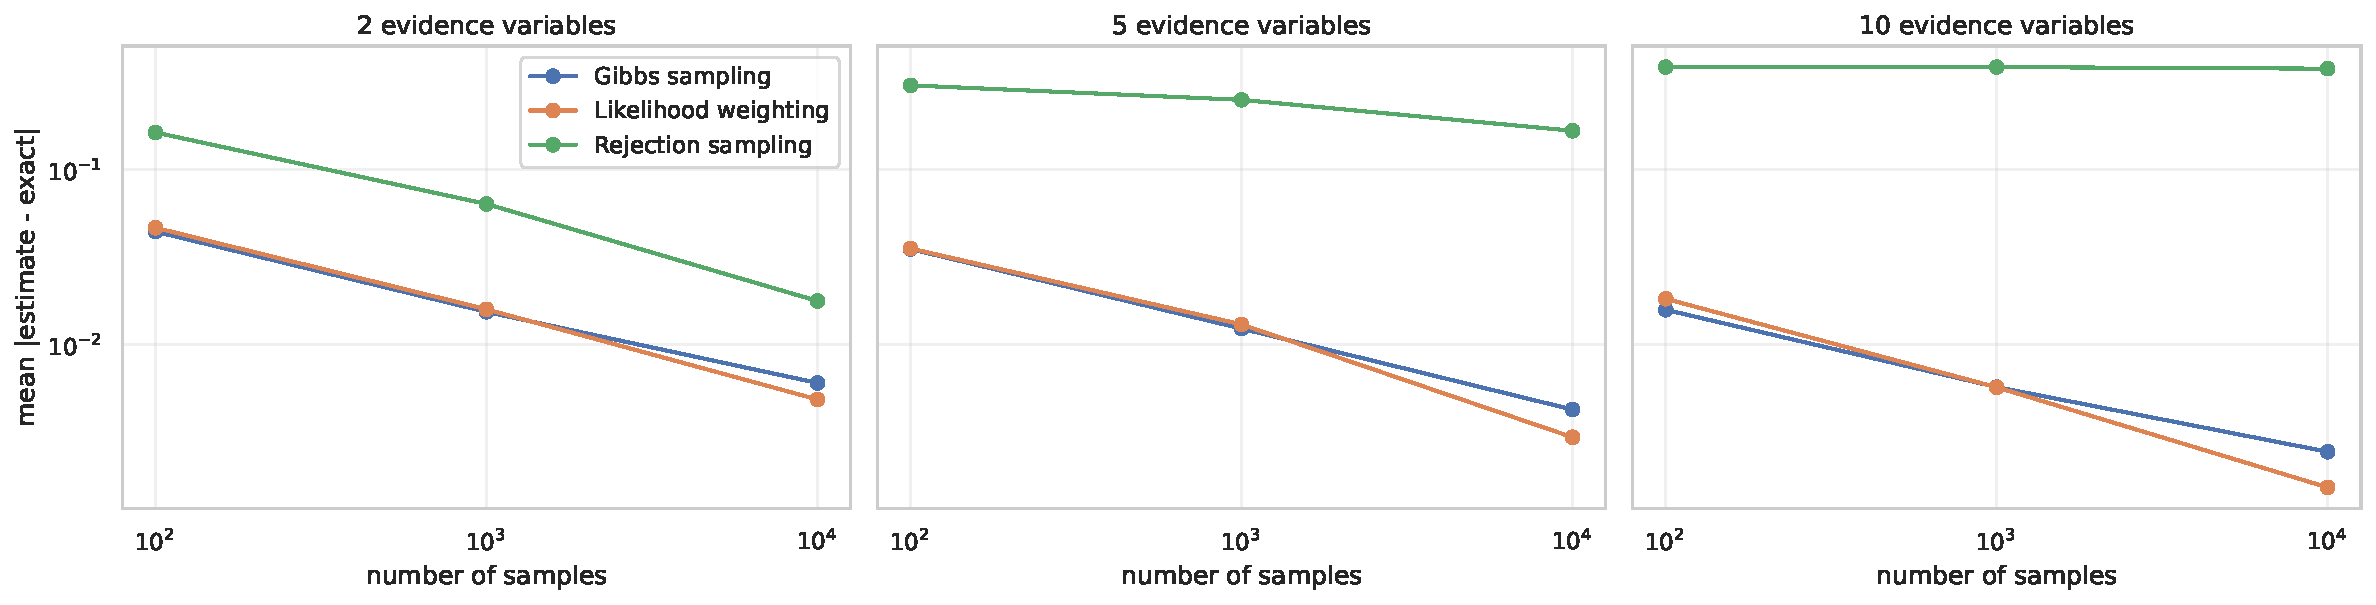
\includegraphics[width=\linewidth]{bn_inference_error.pdf}\caption{Inference.}\label{fig:bn_inference}\end{figure}

\subsection{Overall}
\begin{table}[H]
\centering
\small
\begin{adjustbox}{max width=\linewidth}
\begin{tabular}{llrrrrrr}
\toprule
family & model & pr\_auc & roc\_auc & f2 & recall & precision & accuracy \\
\midrule
Traditional & Hist. Gradient Boosting & \textbf{0.9045} & \textbf{0.9459} & \textbf{0.8132} & \textbf{0.8512} & 0.6901 & 0.8839 \\
Traditional & Random Forest & 0.8934 & 0.9361 & 0.8021 & 0.8068 & 0.7841 & 0.9092 \\
Traditional & Decision Tree & 0.8623 & 0.9180 & 0.7670 & 0.7856 & 0.7006 & 0.8797 \\
Deep learning & MLP (entity embeddings) & 0.8619 $\pm$ 0.0017 & 0.9200 $\pm$ 0.0017 & 0.7621 $\pm$ 0.0017 & 0.7956 $\pm$ 0.0088 & 0.6535 $\pm$ 0.0283 & 0.8626 $\pm$ 0.0105 \\
Deep learning & TabNet & 0.8612 $\pm$ 0.0026 & 0.9180 $\pm$ 0.0014 & 0.7568 $\pm$ 0.0039 & 0.7984 $\pm$ 0.0170 & 0.6288 $\pm$ 0.0398 & 0.8517 $\pm$ 0.0148 \\
Traditional & SVM (RBF) & 0.8561 & 0.9147 & 0.7703 & 0.8117 & 0.6398 & 0.8589 \\
Traditional & k-NN & 0.8163 & 0.8925 & 0.7501 & 0.7906 & 0.6228 & 0.8495 \\
Bayesian network & BN - TAN & 0.7895 & 0.8900 & 0.7390 & 0.8110 & 0.5453 & 0.8108 \\
Bayesian network & BN - Expert DAG & 0.7822 & 0.8712 & 0.7152 & 0.7736 & 0.5493 & 0.8117 \\
Traditional & Logistic Regression & 0.7512 & 0.8797 & 0.7360 & 0.7955 & 0.5665 & 0.8222 \\
Traditional & Linear SVM & 0.7443 & 0.8774 & 0.7339 & 0.7962 & 0.5589 & 0.8180 \\
Bayesian network & BN - Hill-climb BIC & 0.7332 & 0.8579 & 0.7033 & 0.7941 & 0.4826 & 0.7688 \\
Bayesian network & BN - Naive Bayes & 0.7061 & 0.8635 & 0.7149 & 0.7962 & 0.5076 & 0.7866 \\
Traditional & Gaussian Naive Bayes & 0.6244 & 0.8503 & 0.7140 & 0.8096 & 0.4850 & 0.7704 \\
\bottomrule
\end{tabular}
\end{adjustbox}
\caption{All model families on the test set, ranked by PR-AUC (F2, recall, precision and accuracy at the tuned threshold); deep models are mean $\pm$ sd over 5 seeds.}
\label{tab:overall}
\end{table}

\begin{figure}[H]\centering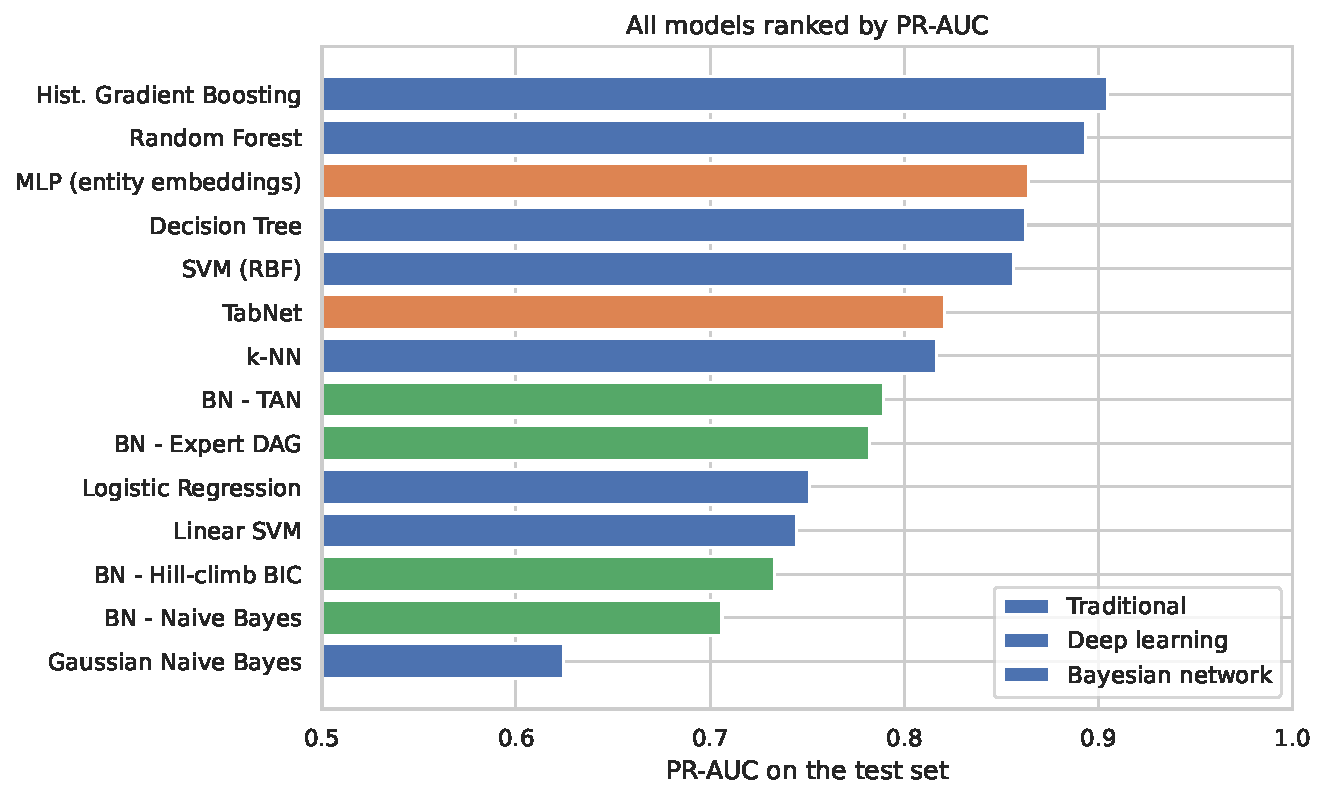
\includegraphics[width=0.8\linewidth]{overall_pr_auc.pdf}\caption{Overall.}\label{fig:overall}\end{figure}
Best: \BestModel{} \BestPrAuc{} \BestFTwo{} \BnBins{} \VeMs{}.

\section{Discussion}
\label{sec:discussion}

\subsection{Comparison of the three approaches}
\Cref{tab:approaches} summarizes the strengths and weaknesses observed for the three families.

\begin{table}[H]
  \centering
  \small
  \begin{tabularx}{\linewidth}{l>{\raggedright\arraybackslash}X>{\raggedright\arraybackslash}X}
    \toprule
    \textbf{Approach} & \textbf{Strengths} & \textbf{Limitations} \\
    \midrule
    Traditional pipeline &
    Best accuracy (gradient boosting); fast to train (seconds); every preprocessing decision is explicit and testable; mature tooling for tuning and thresholding &
    Linear and distance-based models depend heavily on hand-made preprocessing; ensembles are harder to explain than a single model \\
    Deep learning &
    Learns representations of categorical variables end to end; beats every linear model without manual interaction terms; the learned embeddings are reusable features &
    Below the tree ensembles on this medium-sized table; many training hyper-parameters; slower (TabNet especially); less transparent \\
    Bayesian network &
    Explicit, inspectable assumptions; exact answers to any conditional query, in both predictive and diagnostic directions; native handling of missing features &
    Requires discretization, which loses information; CPT size grows exponentially with the number of parents; weakest classifier of the three families \\
    \bottomrule
  \end{tabularx}
  \caption{Strengths and limitations of the three model families on this problem.}
  \label{tab:approaches}
\end{table}

\subsection{What mattered most}
Three decisions had a large effect, and most others had almost none.
\begin{enumerate}
  \item \textbf{The model family.} Moving from a linear model to a tree ensemble raised the test PR-AUC from 0.75 to 0.90, more than every preprocessing choice combined.
  \item \textbf{Scaling, for distance- and margin-based models.} It decides whether k-NN and the SVM are usable at all.
  \item \textbf{The decision threshold.} For a fixed model, moving the threshold trades recall against precision far more than any re-weighting or resampling strategy does. Tuning it for F2 is a direct, transparent way to encode the higher cost of a missed defaulter.
\end{enumerate}
In contrast, the imputation method, the treatment of the seven impossible values, the scaler variant and the resampling method changed PR-AUC by less than the fold-to-fold noise.
Reporting these negative results matters: they show which parts of the pipeline deserve attention in practice.

\subsection{Choice of metric}
Accuracy would have been misleading for this problem.
For example, the random forest has a higher test accuracy than gradient boosting at their tuned thresholds, but a lower recall; a lender who cares about missed defaulters should prefer the latter.
PR-AUC ranks models by how well they separate defaulters across all thresholds, and F2 makes the cost asymmetry explicit when choosing one threshold.
The weight $\beta = 2$ is itself a business assumption: a lender with a different ratio between the cost of a default and the lost margin of a rejected applicant should choose a different $\beta$, or minimize the expected cost directly.

\subsection{Limitations and threats to validity}
\begin{itemize}
  \item \textbf{One dataset and one split.} All conclusions come from one public dataset with a single stratified test split. Cross-validation on the training set agrees with the test results, but the dataset's provenance (country, period, lender) is undocumented, so the absolute numbers may not transfer to other portfolios.
  \item \textbf{No temporal information.} Credit models are normally validated on later loans than they are trained on. The dataset has no dates, so a random split may slightly overstate performance under drift.
  \item \textbf{Limited search spaces.} The grids are deliberately small to keep \emph{Run all} within the limits of a free Colab session. The headroom experiment (\cref{tab:headroom}) suggests this does not change the conclusions for the best family, but other families might gain somewhat from wider searches.
  \item \textbf{Fixed choices.} The IQR factor $k = 1.5$, the four engineered features, the MLP training schedule and the Bayesian-network parent limit were set by convention rather than tuned.
  \item \textbf{Fairness.} The features include age, and home ownership acts as a proxy for wealth. A deployed credit model must be audited for disparate impact, which is outside the scope of this assignment.
  \item \textbf{Calibration.} Class weights and threshold tuning shift the predicted probabilities, so the scores should be calibrated before they are read as default probabilities, for example to price a loan.
\end{itemize}

\section{Conclusion and future work}
\label{sec:conclusion}

This project built and compared three complete approaches to predicting loan default on the Credit Risk Dataset.

The \textbf{traditional pipeline} is fully configurable, from imputation to the classifier, and every option was evaluated with controlled cross-validated ablations.
Scaling decides the fate of distance- and margin-based models, engineered features, IQR clipping and a one-hot grade help the linear models, and PCA and univariate feature selection never help reliably on this low-dimensional table.
After tuning, histogram-based gradient boosting is the best model, with a test PR-AUC of \BestPrAuc{}.
At its F2-tuned threshold it detects \BestRecall{} of the defaulters with a precision of \BestPrecision{}.
A wider hyper-parameter search and a stacked ensemble did not improve on it, which indicates that the result is close to what these features allow.

The \textbf{deep learning pipeline} with entity embeddings outperforms every linear model and produces reusable learned features, but it stays below the tree ensembles, in line with the literature on tabular data.

The \textbf{Bayesian network}, implemented from scratch for the talented-engineering extension, is the least accurate classifier but the most transparent model.
TAN is the best structure for prediction, whereas a better model of the joint distribution, as learned by hill climbing on BIC, does not translate into better classification; comparing exact query answers with empirical frequencies exposes the independence assumptions of each structure.
The inference experiments reproduce the textbook behaviour: variable elimination is exact and fast on these small networks, likelihood weighting and Gibbs sampling converge, and rejection sampling collapses once many variables are observed.

\paragraph{Future work.}
\begin{itemize}[nosep]
  \item Calibrate the probabilities (isotonic or Platt scaling) and choose the threshold by minimizing an explicit expected loss.
  \item Explain individual decisions with SHAP values, as lenders must justify rejections.
  \item Audit the model for disparate impact across age groups.
  \item Learn Bayesian-network parameters with expectation maximization over the incomplete rows, and try continuous (conditional Gaussian) nodes to avoid discretization.
  \item Validate on a time-ordered split if dated loan data become available.
\end{itemize}


\clearpage
\bibliographystyle{plain}
\bibliography{refs/references}

\clearpage
\appendix
\section{Project structure and usage}
\label{app:structure}

\begin{listing}[H]
  \begin{minted}[fontsize=\footnotesize, frame=lines]{text}
notebooks/credit_risk_pipeline.ipynb   Colab front-end (Run all)
modules/creditrisk/
  config.py        paths, dataset URL, column roles, random seed
  data.py          download, rule-based cleaning, stratified split
  eda.py           EDA tables and figures
  transformers.py  grade-wise imputer, IQR clipper, feature engineering
  pipeline.py      PipelineConfig -> scikit-learn / imbalanced-learn Pipeline
  experiments.py   ablation suites, grid search, threshold tuning, test evaluation
  evaluation.py    metrics, cross-validation, ROC / PR / confusion plots
  deep.py          entity-embedding MLP (PyTorch) and TabNet wrapper
  reporting.py     .npy / .h5 feature export, LaTeX tables
  bayesnet/        graph, factor, network, structure, inference, discretize
features/          saved feature sets (.npy) and credit_features.h5
reports/           report.pdf, LaTeX source, figures, generated tables
results/           CSV result of every experiment
tests/             pytest unit tests
  \end{minted}
  \caption{Repository layout.}
  \label{lst:layout}
\end{listing}

\paragraph{Running.}
On Google Colab, open the notebook link from \cref{sec:intro} and choose \emph{Runtime} $\to$ \emph{Run all}.
Locally, install \code{requirements.txt} and PyTorch, then execute the notebook with Jupyter.
The report is compiled with \code{latexmk -pdf -shell-escape report.tex} in \code{reports/latex}.

\section{Unit tests}
\label{app:tests}
The package ships 21 \code{pytest} tests.
They run in a few seconds and cover the following properties.
\begin{itemize}[nosep]
  \item The DAG rejects cycles, and its topological order and Markov blankets are correct.
  \item Variable elimination equals brute-force enumeration on random multi-parent networks, for queries with and without evidence (tolerance $10^{-12}$).
  \item Rejection sampling, likelihood weighting and Gibbs sampling converge to the exact posterior (tolerance 0.01).
  \item Parameter learning recovers the generating CPTs from \num{200000} samples.
  \item A Naive Bayes network gives the same posteriors as scikit-learn's \code{CategoricalNB}.
  \item Missing evidence is marginalized correctly.
  \item TAN and hill climbing produce valid DAGs, and the BIC trace is monotone.
  \item Cleaning, the grade-wise imputer and the IQR clipper behave as specified.
  \item Six representative pipeline configurations fit and predict, and invalid configurations are rejected.
\end{itemize}

\section{Saved feature files}
\label{app:features}
\Cref{tab:features} lists the feature sets written by the notebook.
Every set is stored as separate \code{.npy} arrays and also inside the single file \code{features/credit_features.h5}, with one HDF5 group per set.

\begin{table}[H]
  \centering
  \small
  \begin{tabularx}{\linewidth}{lX}
    \toprule
    \textbf{Folder / HDF5 group} & \textbf{Content} \\
    \midrule
    \code{traditional_logreg} & Output of the tuned logistic-regression preprocessing (imputed, engineered, clipped, one-hot, standardized), with feature names in \code{meta.json} \\
    \code{traditional_<best>} & Output of the preprocessing of the best traditional model \\
    \code{traditional_pca95} & PCA projection retaining 95\% of the variance, with explained-variance ratios \\
    \code{deep_mlp_embeddings} & 64-dimensional penultimate-layer representation of the reference MLP \\
    \bottomrule
  \end{tabularx}
  \caption{Extracted feature sets (\code{X_train}, \code{X_test}, \code{y_train}, \code{y_test} in each).}
  \label{tab:features}
\end{table}


\end{document}
